\documentclass[12pt, oneside,openright]{report} %Letter,
\usepackage[colorlinks=true, linkcolor=black, citecolor=blue, urlcolor = blue, hypertexnames=false]{hyperref}
\usepackage[left=2.54cm, right=2.54cm, top=2.54cm, bottom=2.54cm]{geometry}
\usepackage[spanish]{babel}
\usepackage{parskip}
\usepackage[table]{xcolor}
\usepackage{algpseudocode}
\usepackage[T1]{fontenc}
\usepackage{lmodern}
\usepackage{algorithm}
\usepackage{fancyhdr}
\usepackage{setspace}
\usepackage[utf8]{inputenc}
\usepackage{pdfpages}
\usepackage{csquotes}
\usepackage{multirow}
\usepackage{listings}
\usepackage{graphics}
\usepackage{amsfonts}
\usepackage{graphicx}
\usepackage{amssymb}
\usepackage{amsmath}
\usepackage{amsthm}
\usepackage{epsfig}
\usepackage{subfig}
\usepackage{anyfontsize}
\usepackage{dirtytalk}
\usepackage{array}
\usepackage{tabularx}
\usepackage{textcomp}
\usepackage[backend=biber,style=ieee,sorting=none]{biblatex}
\addbibresource{capitulos/Referencias.bib}

\clubpenalty=10000
\widowpenalty=10000
\displaywidowpenalty=10000
    
\lstdefinestyle{mystyle}{
  keywordstyle=\color{blue},
  basicstyle=\ttfamily\footnotesize,
  breakatwhitespace=false,         
  breaklines=true,                 
  captionpos=b,                    
  keepspaces=true,                                 
  showspaces=false,                
  showstringspaces=false,
  showtabs=false,                  
  tabsize=1
}\lstset{style=mystyle}


\newtheorem{definition}{Definición}
\newtheorem{theorem}{Teorema}

\renewcommand{\lstlistingname}{Codigo}

\renewcommand{\algorithmicrequire}{\textbf{Input:}}
\renewcommand{\algorithmicensure}{\textbf{Output:}}
\renewcommand{\lstlistlistingname}{Índice de Códigos}

\newenvironment{dedicatoria}
    {\newpage \thispagestyle{plain} \vspace*{\stretch{1}}
    \begin{flushright}
    \begin{minipage}{0.9 \textwidth} % Ajusta el ancho aquí
    \em \textbf{Dedicatoria.}
    \vspace{1cm}}
    {\end{minipage}
    \end{flushright}
    \vspace*{\stretch{2}}
    \newpage}
    
% \newenvironment{agradecimientos}
%   {\cleardoublepage\thispagestyle{plain}\vspace*{\stretch{1}}\begin{center}\bfseries Agradecimientos\end{center}}
%   {\vspace*{\stretch{2}}}

\newenvironment{agradecimientos}
  {\cleardoublepage\thispagestyle{plain}\vspace*{\stretch{1}}\begin{center}\bfseries\itshape\fontsize{16pt}{16pt}\selectfont Agradecimientos.\end{center}}
  {\vspace*{\stretch{2}}}

\newenvironment{resumen}
  {\cleardoublepage\thispagestyle{plain}\vspace*{\stretch{1}}\begin{center}\bfseries Resumen.\end{center}}
  {\vspace*{\stretch{2}}}

\newenvironment{_abstract1}
  {\cleardoublepage\thispagestyle{plain}\vspace*{\stretch{1}}\begin{center}\bfseries Abstract1\end{center}}
  {\vspace*{\stretch{2}}}
% \makeatletter

% \makeatother

\makeatletter
\renewcommand*\l@section{\@dottedtocline{1}{1.5em}{4.5em}}
\renewcommand*\l@subsection{\@dottedtocline{2}{3.8em}{5.0em}}
\makeatother
\begin{document}

\makeatletter
  \renewcommand{\ALG@name}{Algoritmo}
\makeatother
  
\renewcommand{\listtablename}{Índice de tablas}
\renewcommand{\tablename}{Tabla}

\begin{titlepage}
\begin{minipage}[l]{3.5cm}

\includegraphics[width=5cm, height=22.0cm]{imagenes/Imagen_front_UPTex.jpg}
\end{minipage}
\vspace*{-3.0cm}
\begin{minipage}[r]{13.0cm}
\begin{center}
\textbf{\LARGE{UNIVERSIDAD POLIT\'{E}CNICA }}\\
\vspace*{0.5cm}
\textbf{\LARGE{DE TEXCOCO}} \\
\vspace*{2.0cm}
\large{\textbf{Análisis estadístico para área de dirección académica escolar}}\\

\vspace*{0.5cm}
\large{\textbf{T E S I S}} \\
\vspace*{0.5cm}
\textbf{Requisito parcial para obtener el  t\'{i}tulo de:}\\
\textbf{INGENIERO(A) EN SISTEMAS COMPUTACIONALES}\\
\vspace*{1.0cm}
\textbf{P R E S E N T A:} \\
\vspace*{0.5cm}
\textbf{Colmenero Lopez Jose Eduardo} \\
\textbf{Leon Sanchez Emiliano} \\

\vspace*{1.0cm}
\textbf{DIRECTOR DE TESIS} \\
\vspace*{0.5cm}
\textbf{Rodriguez Muñoz Octavio}\\
\textbf{}\\
\vspace*{1.0cm}
%\textbf{CODIRECTORES} \\
\vspace*{0.5cm}
%\textbf{GRADO, MAESTRO, DR.} \\
%\textbf{DR. JUAN PEREZ}\\
\vspace*{1.5cm}
TEXCOCO, EDO. MÉX. \hspace{2cm}SEPTIEMBRE 2026 \\
\end{center}
\end{minipage}
\end{titlepage}
\setstretch{1.5}   
\pagenumbering{Roman} \setcounter{page}{2}

\begin{center}


    {\Huge  Análisis estadístico para área de dirección académica escolar}
\end{center}
\vspace{3cm}
Tesis realizada por Colmenero López José Eduardo y León Sánchez Emiliano bajo la dirección del Comité Asesor indicado, aprobada por el mismo y aceptada como requisito parcial para obtener el título de:
\vspace{2cm}

\begin{center}
    {\textbf{ \large{INGENIERO(A) EN SISTEMAS COMPUTACIONALES}}}
\end{center}


\vspace{4cm}

\textit{DIRECTOR: Luna Becerril Edurneth}

\textit{CODIRECTOR:Miguel Sanchez Gerardo}

\textit{ASESOR:  Rodriguez Muñoz Octavio}
\newpage
\begin{agradecimientos}
Expreso mi más profundo agradecimiento a mi familia por brindarme la oportunidad de estudiar esta carrera. Siendo sincero, durante mucho tiempo dudé alcanzar este punto y culminar este trabajo de titulación. Agradezco a mis padres por su respaldo incondicional, su dedicación y por acompañarme en cada momento de dificultad y alegría; mi compromiso es seguir superándome día a día para honrar su esfuerzo y alcanzar nuevas metas.

A mis amigos, gracias por su lealtad, compañerismo y afecto a lo largo de estos años. Conservaré siempre el valor de nuestra etapa universitaria: las conversaciones, los desvelos de estudio y el apoyo constante que me impidió rendirme ante las adversidades académicas. Gracias por estar presentes en las buenas y en las malas, y por ser parte fundamental de mi aprendizaje; les deseo el mayor de los éxitos en cada uno de sus caminos.

Finalmente, a mis hermanas y a mi mascota. Su presencia fue un refugio indispensable en los instantes de desánimo y su alegría ante cada materia superada fue un motor para no abandonar. Gracias por recibirme siempre con los brazos abiertos y por creer en mí incluso en las etapas en que dudé de mis propias capacidades, permitiéndome concluir hoy esta carrera profesional.\\

\textbf{Colmenero López José Eduardo}
\end{agradecimientos}

\begin{agradecimientos}
En primer lugar, quiero agradecer a Dios por concederme cada día el privilegio de vivir y por acompañarme en este camino; Él sabe cuánto esfuerzo y sacrificio ha costado llegar hasta aquí, y gracias a su guía hoy alcanzo esta meta, pues siempre me escuchó cuando lo necesité y jamás me dejó solo. A mi familia, por brindarme siempre su respaldo incondicional, sus enseñanzas y el impulso constante para sacar adelante esta carrera profesional.

A mis amigos, por compartir cada una de las mañanas de desvelo, las intensas tardes de entrega de proyectos y las largas noches de estudio; gracias a quienes estuvieron presentes desde el primer día hasta el último de estos cuatro años, por enseñarme a encontrarle el lado positivo y alegre a cada reto y por esa fraternidad sincera que conservamos día con día.

Y a mis estimados profesores, que supieron comprender nuestras circunstancias como estudiantes y honraron su noble profesión al guiarnos con paciencia, sabiduría y dedicación para formarnos como ingenieros preparados para momentos tan significativos como este.\\

\textbf{León Sánchez Emiliano}
\end{agradecimientos}

\newpage
\begin{dedicatoria}
{

Dedico este trabajo de titulación a mi familia y a mis padres, por su sacrificio y fe inquebrantable que hicieron posible este camino. A mis amigos, por el compañerismo sincero en las buenas y en las malas durante cada etapa universitaria. A mis hermanas y a mi mascota, por ser el hogar cálido que disipó mis dudas y celebró cada avance cuando más lo necesité.
Finalmente, me dedico esta obra a mí mismo. A mis desvelos, a mis sacrificios y a la perseverancia con la que enfrenté cada obstáculo. Hoy reconozco el valor de haberme levantado en los momentos de incertidumbre y de haber creído en mi capacidad para concluir esta carrera. Celebro esta primera gran victoria personal y la tomo como el cimiento de todos los éxitos y metas que están por venir.\\

-Colmenero Lopez Jose Eduardo
}

\end{dedicatoria}

\begin{dedicatoria}
{

A mi por estar estos 4 años luchando con el pensamiento de tener que terminar la carrera y estudiar lo que me gusta, por que, si me gusta todo esto pero uno nunca termina ni de conocerse a si mismo y descubrir nuevas ambiciones, gustos y disgustos, de todas maneras son muy pocos a quienes no les gusta la tecnologia y al final lo que empezo como un simple gusto por la tecnologia y videojuegos, se convirtio en una pequeña ambicion por descubrir todo el mundo que hay detras de la palabra "Tecnologia".
Para toda mi familia por el apoyo incondicional y los valores que me inculcaron y por ser mi soporte en todo momento.
Y por ultimo a mis angelitos que me cuidan desde el cielo, que en vida no me ven ahora pero estoy seguro que estan viendo en todo lo que alcance y la persona que soy ahora.\\

-León Sánchez Emiliano
}

\end{dedicatoria}

\newpage
\section*{Resumen}

La gestión y consolidación de grandes volúmenes de datos históricos en la Dirección Académica de la Universidad Politécnica de Texcoco ha representado un desafío crítico para la toma de decisiones estratégicas. El manejo disperso de la información mediante hojas de cálculo manuales generaba retrasos operativos, inconsistencias en los registros y dificultaba el seguimiento longitudinal de indicadores clave como la matrícula estudiantil, el aprovechamiento académico, la reprobación, la deserción, la eficiencia terminal y los índices de titulación generacional. Para resolver esta problemática, el presente trabajo de titulación describe el diseño, desarrollo, validación y despliegue de una Plataforma Web de Análisis Estadístico Académico, concebida como una solución centralizada y segura para la ingestión, validación, procesamiento analítico y visualización interactiva de series históricas de datos institucionales.

La plataforma fue desarrollada bajo una arquitectura desacoplada de microservicios contenerizados con Docker y guiada por la metodología ágil Kanban. El backend fue implementado con FastAPI sobre Python 3.12, integrando procesamiento asíncrono en segundo plano con Celery y Redis, y persistencia relacional transaccional en PostgreSQL 16 normalizada mediante SQLAlchemy 2.0 y migraciones con Alembic. El frontend se estructuró como una aplicación de una sola página (SPA) responsiva con React 18, TypeScript, Tailwind CSS y Apache ECharts, gestionando el estado global y asíncrono con Zustand y TanStack Query. El sistema incorpora mecanismos de autenticación y control de acceso basado en roles (RBAC) mediante JSON Web Tokens (JWT) y cifrado criptográfico de contraseñas con Argon2.

Los resultados en el entorno de producción evidencian una reducción sustancial en los tiempos de consolidación analítica, pasando de varios días a respuestas inmediatas en milisegundos con ingestión asíncrona robusta. La suite de pruebas automatizadas alcanzó un 100\% de aprobación en validación de reglas de negocio y cálculo de fórmulas oficiales. Esta plataforma proporciona a las autoridades universitarias una fuente única y confiable de información para la planeación académica, la rendición de cuentas y la mejora continua de la calidad educativa.
\addcontentsline{toc}{chapter}{Resumen}
\newpage
\section*{Abstract}

The management and consolidation of large volumes of historical data within the Academic Directorate of the Universidad Politécnica de Texcoco has posed a significant challenge for strategic decision-making. The traditional, decentralized handling of information through manual spreadsheets caused operational delays, data inconsistencies, and hindered the longitudinal monitoring of key performance indicators such as student enrollment, academic achievement, failure rates, dropout rates, graduation rates, and generational degree attainment. To address this issue, this thesis presents the design, development, validation, and deployment of a Web Platform for Academic Statistical Analysis, conceived as a centralized and secure software solution for data ingestion, schema validation, analytical processing, and interactive visualization of institutional historical series.

The platform was built under a decoupled microservices architecture containerized with Docker and guided by the agile Kanban methodology. The backend was developed using FastAPI on Python 3.12, incorporating asynchronous background processing via Celery and Redis, and transactional relational persistence in PostgreSQL 16 managed through SQLAlchemy 2.0 and Alembic migrations. The frontend was structured as a responsive Single Page Application (SPA) utilizing React 18, TypeScript, Tailwind CSS, and Apache ECharts, with global and asynchronous state management handled by Zustand and TanStack Query. The system integrates secure authentication and Role-Based Access Control (RBAC) powered by JSON Web Tokens (JWT) and cryptographic password hashing with Argon2.

Production results demonstrate a substantial reduction in analytical consolidation time, transitioning from several business days of manual effort to sub-second query responses with robust background data processing. The automated test suite achieved a 100\% pass rate across business rule validation and official formula calculations. This platform provides university authorities with a reliable, single source of truth to support academic planning, institutional accreditation, and the continuous enhancement of educational quality.
\addcontentsline{toc}{chapter}{Abstract}
\newpage 
%\input{capitulos/_resultadosAcademicos}\addcontentsline{toc}{chapter}{Resultados Académicos}
%\newpage

%\begin{spacing}{1.5}
    \tableofcontents
    \newpage
    \listoffigures
    \newpage
    \listoftables
    \newpage
    %\input{acronimos.tex}
%\end{spacing}


\pagenumbering{arabic} \setcounter{page}{1} % Números arábigos para el contenido principal




 La administración educativa moderna requiere de herramientas tecnológicas capaces de transformar datos operativos en información estratégica. El presente documento detalla el diseño y desarrollo de la Plataforma de Análisis Estadístico para la Dirección Académica Escolar, un sistema integral creado para optimizar la toma de decisiones institucionales mediante la automatización y el procesamiento centralizado de datos. El objetivo principal de esta plataforma es agilizar la gestión y el análisis de indicadores académicos críticos. 
 El sistema abarca módulos fundamentales para el entorno escolar, tales como el seguimiento de la matrícula, eficiencia, rendimiento, procesos de titulación, asignación de becas, caracterización estudiantil y evaluaciones docentes. Para proporcionar una perspectiva analítica precisa y evaluar la evolución de la institución, la plataforma consolida y analiza información histórica a un plazo de 3 años hacia el pasado, permitiendo así identificar tendencias, ciclos generacionales y áreas de oportunidad con base en datos reales.  
 A través de una arquitectura robusta —que contempla el procesamiento de datos en segundo plano, validación de cargas masivas de archivos y la generación dinámica de reportes—, el proyecto busca eliminar los cuellos de botella asociados al manejo manual de la información. Los siguientes apartados de este documento profundizan en las especificaciones, requerimientos de software, arquitectura del sistema y las decisiones tecnológicas implementadas para consolidar esta solución en beneficio de la administración escolar.




\section{Antecedentes}

La Dirección Académica de la Universidad Politécnica de Texcoco ha enfrentado históricamente el reto de gestionar un volumen creciente de información escolar sin contar con una herramienta informática centralizada y especializada para el análisis estadístico de sus indicadores clave. 
Tradicionalmente, el almacenamiento y la administración de los datos institucionales se han delegado en hojas de cálculo electrónicas, específicamente archivos de Microsoft Excel. Si bien este método ha sido una solución accesible para el registro inicial de datos, 
la escala operativa de la universidad ha superado las capacidades de esta herramienta, debido a que la información correspondiente a la matrícula, la asignación de becas, el rendimiento, la eficiencia terminal, los ciclos generacionales y los procesos de titulación se encuentra dispersa en múltiples archivos individuales, cada uno estructurado con complejas estructuras de varias hojas de trabajo. 
Esta fragmentación de la información provoca que cuando surge la necesidad de consultar datos específicos o consolidados, el personal académico deba navegar de forma manual a través de decenas de pestañas y archivos independientes, volviendo el proceso de búsqueda y manejo de información sumamente tedioso, propenso a errores humanos y tardado, lo que disminuye drásticamente la capacidad de respuesta institucional. Asimismo, la evaluación del desempeño escolar requiere analizar la evolución académica con una perspectiva de al menos tres años hacia el pasado. 
Realizar este análisis histórico cruzando múltiples hojas de cálculo incrementa exponencialmente el riesgo de duplicidad, pérdida de consistencia en los datos y errores en la aplicación de fórmulas estadísticas, además de impedir la generación dinámica e inmediata de reportes ejecutivos o tableros visuales para los directivos.
\newpage

1. \textbf{Romero Alepuz, J. (2026). Dashboard web para la gestión y visualización dinámica de datos heterogéneos. Universitat Oberta de Catalunya (UOC).}

En este proyecto de titulación se presenta el diseño y desarrollo de un tablero de control (dashboard) web dinámico, el cual fue creado con la finalidad de recopilar y mostrar visualmente información que proviene de diferentes fuentes externas independientes. 
El objetivo principal de este sistema fue ofrecer una herramienta interactiva de autoservicio que funcione como una alternativa viable frente a las plataformas comerciales complejas y a las soluciones estáticas basadas en plantillas tradicionales, permitiendo que los usuarios configuren sus propios paneles de 
indicadores sin la necesidad de contar con conocimientos avanzados de programación. El resultado final de la investigación demuestra la viabilidad de centralizar datos que originalmente se encuentran desordenados o dispersos dentro de un único punto de control seguro, modular y escalable que  
agiliza el monitoreo de la información.


2. \textbf{Andrango, K. (2024). Dashboard estadístico sobre la publicación de datos abiertos por parte de las Instituciones de la Función Ejecutiva en el portal de datos abiertos del Ecuador.}

Este trabajo de titulación se centra en la propuesta y el desarrollo de un panel estadístico diseñado para resolver la falta de control y la poca claridad en la gestión de datos de distintas instituciones públicas. 
La problemática que motivó esta investigación radicaba en que la información se presentaba de forma muy general, lo que impedía supervisar de manera efectiva el cumplimiento y avance real de cada dependencia. 
Para solucionar esto, el autor estructuró un sistema basado en dos reportes clave: el primero reemplaza las cifras generales por una visión específica y detallada que proporciona una representación numérica exacta de los registros; mientras que el segundo reporte funciona 
como un mecanismo de monitoreo integral para rastrear el desempeño de cada institución. El proyecto demuestra cómo un panel de indicadores centralizado promueve la transparencia y facilita la comprensión de grandes volúmenes de información, transformando datos dispersos en informes visuales resumidos
 que apoyan directamente la rendición de cuentas.

\begin{figure}[H]
    \centering
    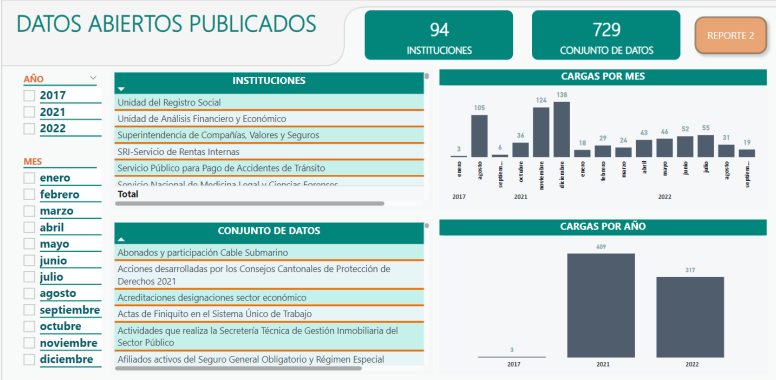
\includegraphics[width=0.8\linewidth]{imagenes/anexo2.png}
    \caption{Dashboard estadístico sobre la publicación de datos abiertos por parte de las Instituciones de la Función Ejecutiva en el portal de datos abiertos del Ecuador}
    \label{fig:dashboard_anexo2}
\end{figure}

3. \textbf{Rangel Narváez, A. (2016). Programación de un Web Dashboard para la presentación de estadísticas en una empresa. Facultad de Ciencias, Universidad Nacional Autónoma de México (UNAM).}

En este proyecto profesional se aborda la necesidad de optimizar la administración de los datos históricos de operación dentro de una organización, partiendo del principio de que esta información es el recurso más valioso para medir el comportamiento de un entorno y guiar su rumbo. 
El autor explica que el almacenamiento tradicional en registros individuales genera serios inconvenientes para el personal, ya que extraer la información requiere conocimientos técnicos avanzados y organizar millones de datos de forma manual vuelve muy lenta la entrega de reportes. 
Para resolver esta situación, se programó una plataforma web interactiva con gráficos, tablas y alertas que consolidan las métricas en un solo lugar con el fin de ofrecer una visión clara para el análisis de operaciones y la toma de decisiones rápidas. El desarrollo demuestra cómo automatizar las rutinas de cálculo para que la información esté actualizada constantemente y disponible para ser consultada a través de internet.
\newpage
4. \textbf{Martínez Luna, I. (2024). Elaboración de un dashboard, aplicado a la minería de datos para el apoyo a la toma de decisiones en el departamento de ventas. Facultad de Estudios Superiores Cuautitlán, UNAM.}

En esta tesis de licenciatura se analiza la problemática de las organizaciones que aún gestionan su información mediante procesos tradicionales y manuales, lo que genera retrasos en la elaboración de reportes, inconsistencia en los datos y poca confiabilidad al momento de evaluar los resultados. 
Para optimizar este flujo de trabajo, el autor implementó una metodología sistemática orientada a descubrir conocimiento dentro de las bases de datos, permitiendo transformar la información cruda en reportes consistentes dirigidos a los altos mandos. 
El proyecto consistió en diseñar un almacén de datos centralizado para reunir la información que se encontraba dispersa en múltiples hojas de cálculo, aplicando un proceso de limpieza para corregir las capturas erróneas antes de realizar la carga final. 
El resultado permite automatizar los informes y aplicar modelos estadísticos avanzados para encontrar patrones, tendencias y proyecciones relevantes representadas en forma gráfica y resumida.

\begin{figure}[H]
    \centering
    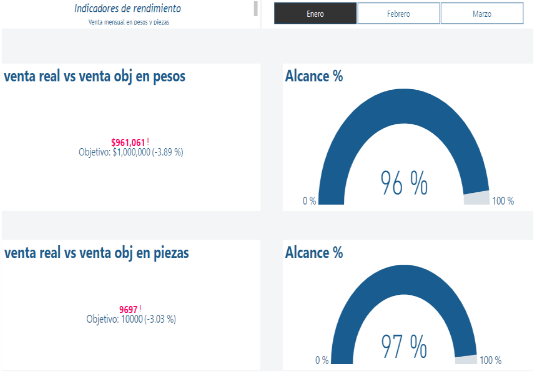
\includegraphics[width=0.8\linewidth]{imagenes/anexo3.png}
    \caption{Dashboard para departamento de ventas}
    \label{fig:dashboard_anexo3}
\end{figure}

\section{Planteamiento del problema}

En la Universidad Politécnica de Texcoco, el área de Dirección Académica tiene la tarea de controlar y revisar datos muy importantes, como la cantidad de alumnos que entran y salen, el rendimiento académico de los estudiantes, la eficiencia terminal, la titulación, las becas y las evaluaciones. 
Toda esta información sirve para que las autoridades de la escuela puedan planear mejoras y saber qué pasos dar en el futuro. 
\begin{figure}[H]
    \centering
    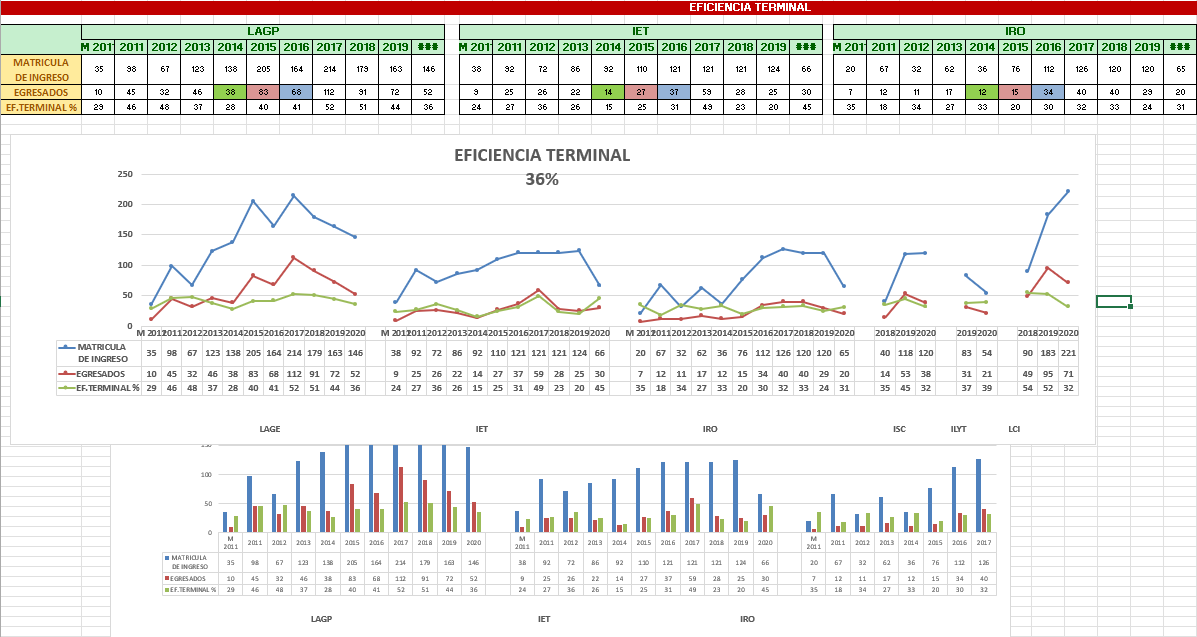
\includegraphics[width=0.8\linewidth]{imagenes/anexo1.png}
    \caption{Análisis de la situación actual}
    \label{fig:situacion_actual_anexo1}
\end{figure}
El gran detalle es que hoy en día todo este registro se hace a mano guardando los datos en archivos de Excel individuales. 
Aunque este sistema ha servido por un tiempo, la realidad es que trabajar así provoca muchos dolores de cabeza: es facilísimo cometer errores al escribir los datos, buscar información se vuelve una tarea muy pesada y las tablas no permiten ver los cambios de forma rápida o directa. 
Esto hace que sea muy difícil notar a tiempo cosas urgentes, como qué alumnos están a punto de dejar la escuela o en qué cuatrimestres específicos los estudiantes están bajando sus calificaciones y necesitan apoyo extra. No contar con un programa moderno e inteligente en la oficina de Dirección Académica frena la posibilidad de vigilar cómo va la universidad día con día. 
En la actualidad, para poder armar un informe o hacer una comparación de datos, el personal tiene que revisar manualmente carpetas llenas de hojas de cálculo, lo que quita muchísimo tiempo y retrasa la entrega de respuestas a los directivos. 
Además, tener la información regada por tantas partes complica juntarla toda en un solo lugar y bloquea la oportunidad de hacer estudios más completos a través de los años, como ver si los cambios que ha hecho la escuela realmente han servido a lo largo del tiempo. Todo esto afecta directamente la administración de la universidad, ya que las decisiones tardan en tomarse y se vuelve muy difícil proponer mejoras basadas en datos reales y ordenados.


\section{Justificación}

La gestión eficiente de la información académica es un factor crítico para el desarrollo y la mejora continua de cualquier institución de educación superior. Cuatrimestre a cuatrimestre, la Universidad Politécnica de Texcoco genera una cantidad masiva de datos vitales, tales como registros de matrícula, índices de reprobación y deserción, tasas de eficiencia terminal y resultados de las evaluaciones docentes. Sin embargo, el almacenamiento y análisis de esta información a través de hojas de cálculo aisladas y archivos de texto plano (CSV) presenta limitaciones significativas. Este manejo manual no solo hace que la consolidación de los datos sea un proceso lento y susceptible a errores humanos, sino que dificulta la visualización rápida de tendencias históricas, retrasando la capacidad de respuesta administrativa.

El desarrollo de este sistema web de indicadores institucionales se justifica por la necesidad imperante de modernizar, centralizar y automatizar el procesamiento de dichos datos. Al implementar una plataforma tecnológica que ingiera directamente los archivos estructurados y los transforme en tableros interactivos (dashboards), se elimina la redundancia operativa y se garantiza la integridad de la información. Esto permitirá a los coordinadores y directivos realizar cruces de información complejos en cuestión de segundos, como comparar el desempeño docente con los índices de aprovechamiento, o consultar el histórico de titulación de las últimas generaciones sin necesidad de buscar en múltiples archivos físicos o digitales.

Además del ahorro sustancial en tiempos de procesamiento administrativo, el mayor impacto de este proyecto radica en su aporte a la toma de decisiones. Dotar a la Universidad Politécnica de Texcoco de una herramienta de inteligencia de datos con control de acceso seguro asegurará que las autoridades cuenten con métricas precisas, actualizadas y fáciles de interpretar. En consecuencia, la institución tendrá una base empírica sólida para fundamentar sus estrategias de retención estudiantil, evaluar la calidad de sus programas educativos, facilitar auditorías y, en última instancia, elevar su nivel de excelencia académica.


 \section{Objetivo General}

Desarrollar un sistema web para el análisis y visualización de indicadores institucionales de la Universidad Politécnica de Texcoco, que permita la ingestión automática de datos académicos y administrativos, su procesamiento mediante rutinas estadísticas, y la representación de resultados con gráficos dinámicos, con el fin de facilitar la toma de decisiones basada en evidencia y mejorar la gestión estratégica de la institución.

\subsection{Objetivos especificos:}

\begin{itemize}
    \item Analizar y estructurar los conjuntos de datos históricos de la institución (archivos CSV de matrícula, aprovechamiento, titulación y evaluación docente) para diseñar el modelo de base de datos relacional que soportará el sistema.
\end{itemize}

 \begin{itemize}
     \item Desarrollar rutinas de procesamiento estadístico y métricas (eficiencia terminal, índice de reprobación, análisis de evaluación docente) capaces de ejecutarse automáticamente tras la carga de nuevos datos, generando indicadores actualizados en tiempo real.
 \end{itemize}

 \begin{itemize}
     \item Implementar una interfaz web responsiva con visualización de datos mediante gráficos interactivos (tableros tipo dashboard) que faciliten la interpretación de indicadores clave y la comparación histórica de métricas institucionales.
 \end{itemize}

 \begin{itemize}
     \item Establecer un sistema de autenticación y perfiles de usuario seguro para restringir el acceso a información sensible y permitir que cada usuario interactúe únicamente con las funcionalidades pertinentes.
 \end{itemize}

 \begin{itemize}
     \item Ejecutar pruebas integrales de rendimiento, validación de datos y usabilidad para verificar que la generación de las gráficas interactivas sea exacta, fluida y cumpla con los requerimientos operativos de la universidad.
 \end{itemize}

 
\chapter{Marco Teórico.}


% ============================================================
\section{Metodología de Desarrollo: Kanban}
\label{sec:metodologia-kanban}
% ============================================================

 \textbf{Kanban} como metodología ágil ligera, fundamentada en la gestión visual del flujo de trabajo \cite{anderson2010}. A diferencia de los marcos que estructuran el desarrollo en iteraciones fijas (\textit{sprints}) como Scrum \cite{scrumguide} o eXtreme Programming \cite{beck2004}, Kanban propone un \textbf{flujo continuo} donde las tareas avanzan de forma progresiva por un tablero visual dividido en columnas que representan los estados del proceso. El término proviene del japonés (\textit{señal visual} o \textit{tarjeta}) y fue concebido originalmente por Toyota en la manufactura para ser posteriormente adaptado a la ingeniería de software por David J. Anderson, quien formuló sus principios y prácticas esenciales \cite{anderson2010}.

\subsection{Principios de Kanban en el Desarrollo de Software}

Los cuatro principios fundamentales de Kanban que guían el desarrollo de software son:

\begin{enumerate}
    \item \textbf{Visualización del flujo de trabajo:} Todas las tareas de un proyecto se representan como tarjetas en un tablero, permitiendo al equipo identificar el estado de avance de cada componente en todo momento.

    \item \textbf{Limitación del trabajo en progreso (WIP --- Work In Progress):} En cada etapa del tablero se limita el número de tareas activas simultáneamente. Esto evita la sobrecarga del equipo y asegura que cada módulo sea completado y validado antes de iniciar el siguiente.

    \item \textbf{Gestión del flujo continuo:} En lugar de planificar iteraciones de duración fija, las tarjetas de trabajo fluyen de manera continua desde su concepción hasta su despliegue, priorizando aquellas funcionalidades con mayor impacto o valor para los usuarios.

    \item \textbf{Mejora continua (Kaizen):} Durante el ciclo de vida del software se realizan revisiones periódicas en las que se analizan cuellos de botella, se corrigen decisiones de diseño y se refinan los procesos de trabajo.
\end{enumerate}

\subsection{Estructura de un Tablero Kanban}

Un tablero Kanban típico se organiza en columnas principales que representan los estados del flujo de trabajo, por ejemplo:

\begin{table}[H]
\centering
\begin{tabular}{|l|p{9cm}|}
\hline
\textbf{Columna} & \textbf{Descripción} \\
\hline
\textbf{Backlog} & Lista priorizada de todas las funcionalidades identificadas en el documento de requerimientos. \\
\hline
\textbf{Análisis} & Tareas en estudio de factibilidad técnica, definición del modelo de datos o diseño de la interfaz. \\
\hline
\textbf{En Desarrollo} & Tarjeta activamente codificada. Límite WIP: 2 tarjetas simultáneas. \\
\hline
\textbf{En Pruebas} & Funcionalidad implementada bajo verificación con pruebas automatizadas (\texttt{pytest}) y revisión manual. \\
\hline
\textbf{Desplegado} & Funcionalidad integrada a la rama principal y disponible en el entorno de producción mediante CI/CD. \\
\hline
\end{tabular}
\caption{Columnas del tablero Kanban.}
\end{table}

\section{Arquitectura y Conceptos Web Modernos}

Los sistemas de software modernos requieren arquitecturas que separen claramente la lógica de presentación de la lógica de procesamiento \cite{fowler2002}. 

\subsection{Aplicaciones de una Sola Página (Single Page Application - SPA)}
Una SPA es una aplicación web que interactúa con el usuario cargando dinámicamente el contenido del navegador en lugar de recargar páginas completas desde el servidor. Este enfoque mejora drásticamente la fluidez de la experiencia del usuario y disminuye el ancho de banda consumido, debido a que toda la estructura de la interfaz (HTML, CSS y JavaScript) se transfiere al inicio del ciclo de navegación. A partir de ese momento, las interacciones posteriores solicitan exclusivamente datos crudos (normalmente en formato JSON) al backend a través de llamadas asíncronas \cite{sommerville2016}.

\subsection{APIs REST (Representational State Transfer)}
Una API REST es un estilo de arquitectura de software diseñado para interconectar sistemas a través del protocolo de transferencia de hipertexto (HTTP), formalizado originalmente por Roy Fielding \cite{fielding2000}. Se fundamenta en recursos identificados mediante URLs únicas y en el uso de los métodos estándar de HTTP (GET, POST, PUT, DELETE) para realizar operaciones. La comunicación REST es por definición "sin estado" (stateless), lo que significa que cada petición del cliente contiene toda la información necesaria para ser procesada por el servidor, simplificando la escalabilidad horizontal del backend.

\subsection{Procesamiento Asíncrono y Concurrencia}
Cuando un sistema maneja operaciones computacionalmente costosas en tiempo de ejecución, como el análisis de archivos Excel masivos o la generación de reportes analíticos complejos, el procesamiento síncrono bloquea el hilo principal de ejecución, degradando severamente el tiempo de respuesta del servidor \cite{kleppmann2017}. La concurrencia asíncrona resuelve esta limitación permitiendo que el servidor inicie una tarea larga y continúe procesando otras solicitudes entrantes sin esperar su finalización. Las tareas de larga duración son delegadas a trabajadores en segundo plano (background workers), mientras el cliente recibe un identificador único para monitorear el estado del proceso mediante peticiones periódicas (polling) o comunicación bidireccional \cite{kleppmann2017}.

\subsection{Mapeo Objeto-Relacional (ORM)}
El Mapeo Objeto-Relacional es un patrón de diseño y técnica de programación que permite traducir los datos almacenados en una base de datos relacional (tablas y registros) a objetos en el lenguaje de programación orientado a objetos, facilitando la interacción con la base de datos sin escribir sentencias de SQL de forma manual \cite{fowler2002}. El ORM proporciona abstracción sobre el motor de base de datos específico, protegiendo al sistema contra vulnerabilidades críticas como la inyección de código SQL mediante la parametrización y escape automático de consultas.



\section{Tecnologías del Backend}

El backend actúa como la capa de procesamiento y lógica de negocios en una arquitectura web. Dentro del ecosistema de Python, existen diversas herramientas para lograr un alto rendimiento y una ejecución asíncrona robusta \cite{python2024, ramirez2024}.

\subsection{Python 3.12}
Python es un lenguaje de programación de alto nivel, interpretado y multiparadigma, ampliamente utilizado en el ámbito del análisis de datos y la ingeniería de software debido a su sintaxis legible y a su extenso ecosistema de bibliotecas científicas. La versión 3.12 introduce mejoras significativas en el recolector de basura, optimización de velocidad de ejecución en el intérprete CPython y soporte mejorado para tipos genéricos y tipado estático opcional (Type Hints), permitiendo escribir código más legible, seguro y con menor consumo de memoria en tareas que demandan un alto procesamiento numérico \cite{python2024}.

\subsection{FastAPI}
FastAPI es un framework moderno de alto rendimiento diseñado para construir APIs con Python utilizando el tipado estándar del lenguaje \cite{ramirez2024}. Su excelente rendimiento es atribuible al uso de Starlette para las capacidades web y Pydantic para la serialización y validación de datos. FastAPI proporciona soporte nativo para programación asíncrona mediante las sentencias \texttt{async} y \texttt{await}, permitiendo al servidor manejar miles de peticiones simultáneas con baja latencia. Adicionalmente, genera de manera automática la documentación interactiva de la API bajo el estándar OpenAPI.

\subsection{SQLAlchemy 2.0 (Async)}
SQLAlchemy es un toolkit de SQL y un ORM para Python que proporciona potencia y flexibilidad en el acceso a bases de datos relacionales \cite{bayer2024}. La versión 2.0 reescribe la arquitectura del ORM para soportar completamente la ejecución asíncrona de manera nativa con drivers no bloqueantes como \texttt{asyncpg}. Esto evita que las llamadas a la base de datos bloqueen el bucle de eventos (event loop) de FastAPI, optimizando el rendimiento de la aplicación en entornos multiusuario concurrentes.

\subsection{Alembic}
Alembic es la herramienta oficial de migraciones de bases de datos para SQLAlchemy \cite{alembic2024}. Permite gestionar la evolución del esquema de la base de datos a lo largo del tiempo, registrando cronológicamente cada modificación estructural (creación de tablas, nuevas columnas o índices) mediante archivos de migración escritos en Python. Esto garantiza la sincronización del modelo de datos de la aplicación con la base de datos física en los entornos de desarrollo, pruebas y producción de forma automática y reproducible.

\subsection{Pandas}
Pandas es la biblioteca estándar en la industria para el análisis y manipulación de datos en Python \cite{mckinney2010, mckinney2022}. Mediante el uso de estructuras de datos optimizadas en memoria llamadas DataFrames, Pandas permite leer, indexar, agrupar, filtrar y limpiar grandes volúmenes de datos provenientes de archivos tabulares como CSV y hojas de cálculo de Excel de manera extremadamente rápida. En el desarrollo de software orientado a datos, Pandas suele utilizarse como el motor principal para procesar, limpiar y transformar la información antes de ser cargada a una base de datos relacional.

\subsection{Celery}
Celery es una biblioteca para Python que implementa una cola de tareas asíncronas basada en el paso de mensajes distribuidos \cite{solem2024}. Se enfoca en operaciones en tiempo real, soportando también la programación de tareas periódicas. Celery permite desacoplar los procesos computacionalmente costosos del flujo principal de ejecución web. Cuando se recibe una solicitud pesada, el servidor web registra el trabajo en Celery y responde de inmediato al cliente, mientras que un proceso worker independiente ejecuta la tarea compleja en segundo plano sin interrumpir la disponibilidad del sistema general.



\section{Tecnologías del Frontend}

El frontend es la capa responsable de interactuar con el usuario final, presentar de manera visual la información estructurada y capturar los datos de entrada a través de interfaces dinámicas y accesibles \cite{sommerville2016, react2024}.

\subsection{React 18}
React es una biblioteca de JavaScript orientada a la creación de interfaces de usuario interactivas basadas en componentes reutilizables \cite{react2024}. React 18 introduce características clave como la renderización concurrente, que permite al navegador pausar y reanudar la actualización de los elementos visuales para mantener la fluidez en pantallas con alta carga computacional (como las gráficas estadísticas). Utiliza un modelo de representación en memoria llamado Virtual DOM para minimizar las operaciones de manipulación directa sobre el navegador, mejorando la velocidad de respuesta del frontend.

\subsection{TypeScript}
TypeScript es un lenguaje de programación de código abierto desarrollado por Microsoft que actúa como un superconjunto estricto de JavaScript, añadiendo tipos estáticos opcionales al lenguaje \cite{bierman2014}. El uso de TypeScript en el desarrollo del frontend ayuda a detectar errores de concordancia de datos en tiempo de compilación y proporciona autocompletado avanzado durante la programación de las vistas y flujos de datos. Esto asegura que la comunicación entre la API del backend y las vistas de React comparta exactamente las mismas interfaces y modelos estructurados de datos.

\subsection{Vite}
Vite es una herramienta moderna de construcción y empaquetamiento de aplicaciones frontend \cite{you2024}. A diferencia de las herramientas tradicionales que pre-empaquetan todo el código del proyecto antes de levantar el servidor de desarrollo, Vite aprovecha el soporte nativo de módulos ES (ESM) en los navegadores modernos para servir el código fuente de forma instantánea. Su compilador en segundo plano, escrito en lenguajes compilados de bajo nivel (Go), reduce el tiempo de inicio de la aplicación y agiliza las actualizaciones en caliente (Hot Module Replacement - HMR) durante el desarrollo local.

\subsection{Tailwind CSS}
Tailwind CSS es un framework de hojas de estilo (CSS) basado en clases de utilidad de bajo nivel \cite{wathan2024}. En lugar de proporcionar componentes visuales preestablecidos y difíciles de personalizar, Tailwind ofrece clases atómicas que controlan de manera directa el margen, espaciado, colores, tipografía y diseño adaptivo (responsive) directamente en el código de marcado de React. Esto evita la escritura de archivos CSS adicionales y reduce drásticamente el peso final de los archivos estáticos compilados para producción.

\subsection{Apache ECharts}
Apache ECharts es una biblioteca de visualización de datos potente, interactiva y de código abierto escrita en JavaScript \cite{echarts2018}. Está optimizada para renderizar millones de puntos de datos de forma fluida mediante el uso de elementos vectoriales (SVG) o mapas de bits dinámicos (Canvas). Esta herramienta se implementa habitualmente para renderizar gráficos de barras, líneas temporales y diagramas de dispersión necesarios para ilustrar de forma interactiva información analítica o estadística compleja.

\subsection{TanStack Query (React Query)}
TanStack Query es una biblioteca declarativa de gestión de estado para aplicaciones React que simplifica el proceso de obtención, almacenamiento en caché, sincronización y actualización de datos asíncronos provenientes del backend \cite{linsley2024}. Elimina la necesidad de escribir estados locales redundantes para manejar el estado de carga (loading), error o éxito de las peticiones HTTP, y actualiza de forma transparente los componentes visuales mediante estrategias inteligentes de invalidación de caché.

\subsection{Zustand}
Zustand es una biblioteca ligera de gestión de estado global para React basada en hooks \cite{kato2024}. Se caracteriza por su simplicidad sintáctica y por no requerir de arquitecturas complejas de proveedores de contexto (Context Providers). Zustand se utiliza frecuentemente para sincronizar de manera eficiente estados globales (como paneles de filtros o preferencias de usuario) entre diversos componentes independientes dentro de aplicaciones interactivas.



\section{Base de datos, gestión de tareas e infraestructura}

La capa de infraestructura y persistencia provee el almacenamiento robusto de los datos, la mediación de mensajes asíncronos y el entorno controlado de virtualización necesario para la ejecución del software.

\subsection{PostgreSQL 16}
PostgreSQL es un sistema de gestión de bases de datos relacionales objeto-relacional altamente estable y de código abierto \cite{postgresql2024}. Destaca por su estricto cumplimiento de los estándares SQL, consistencia de datos y soporte integral para las propiedades ACID (Atomicidad, Consistencia, Aislamiento y Durabilidad) en entornos de alta concurrencia. La versión 16 incluye mejoras en el rendimiento de consultas lógicas paralelas, soporte avanzado de replicación y compresión de índices, garantizando la persistencia e integridad de las series históricas de los indicadores académicos.

\subsection{Redis 7}
Redis es un almacén de estructura de datos en memoria de código abierto utilizado como base de datos de clave-valor, memoria caché de baja latencia y gestor de mensajes \cite{carlson2013}. Su alta velocidad de lectura y escritura (operando directamente en la memoria RAM del sistema) lo convierte en el broker de mensajería ideal para Celery, sirviendo de puente para almacenar temporalmente los mensajes de tareas pendientes y los resultados generados por los trabajadores en segundo plano de manera segura y concurrente.

\subsection{Docker y Docker Compose}
Docker es una plataforma de software que permite automatizar el despliegue de aplicaciones dentro de contenedores de software ligeros y autónomos \cite{merkel2014}. Los contenedores aíslan la aplicación y sus dependencias (como la versión específica de Python, Node.js y librerías del sistema operativo) para garantizar que el software funcione de manera idéntica en cualquier entorno de hardware. Docker Compose es una herramienta para definir y arrancar aplicaciones multi-contenedor; mediante un archivo YAML simplifica la inicialización simultánea del frontend, backend, workers de Celery, base de datos PostgreSQL y caché Redis bajo una misma red virtual aislada y segura.

\subsection{Nginx}
Nginx es un servidor web y un proxy inverso de alto rendimiento diseñado para manejar de forma concurrente cientos de miles de peticiones HTTP con un bajo consumo de recursos de CPU y memoria \cite{reese2008}. En una infraestructura de producción moderna, Nginx actúa habitualmente como la puerta de acceso principal: se encarga de recibir las conexiones de red, servir directamente y con baja latencia los archivos estáticos generados por herramientas del frontend y redirigir dinámicamente las solicitudes de API hacia el servidor de aplicaciones subyacente de forma segura.



\section{Seguridad y Autenticación}

El control de acceso y la integridad de los sistemas web modernos se fundamentan en esquemas de cifrado y autenticación sin estado basados en estándares de la industria.

\subsection{JSON Web Token (JWT)}
JWT es un estándar abierto (RFC 7519) que define una forma compacta y autónoma de transmitir información estructurada de manera segura entre las partes como un objeto JSON \cite{rfc7519}. La información está firmada digitalmente con una clave criptográfica secreta en el backend, lo que evita que el contenido sea manipulado por terceros. Un esquema de autenticación sin estado común mediante JWT se compone típicamente de:
\begin{itemize}
    \item \textbf{Token de Acceso (Access Token):} Un token de corta duración que se incluye en las cabeceras HTTP de cada consulta para validar los permisos e identidad del usuario.
    \item \textbf{Token de Refresco (Refresh Token):} Un token de mayor duración que se utiliza exclusivamente para solicitar un nuevo token de acceso válido sin forzar al usuario a ingresar sus credenciales nuevamente, reduciendo la exposición a riesgos de robo de identidad.
\end{itemize}

\subsection{Argon2}
Argon2 es una función moderna de hashing criptográfico para contraseñas, seleccionada como la ganadora de la Password Hashing Competition en 2015 y estandarizada bajo la RFC 9106 \cite{rfc9106}. A diferencia de los algoritmos de hashing tradicionales como MD5 o SHA-1, Argon2 está explícitamente diseñado para ser configurable y altamente resistente a ataques de fuerza bruta asistidos por hardware especializado (tarjetas gráficas GPUs o circuitos ASICs) mediante el control parametrizado del consumo de tiempo de CPU y, principalmente, el uso intensivo de bloques de memoria RAM (Memory-Hard Function). Esto garantiza que la información de acceso de los usuarios se encuentre debidamente protegida frente a ataques avanzados orientados a la extracción de contraseñas.

\chapter{Desarrollo}
En este capítulo se detalla el proceso de construcción del sistema SIVEH, partiendo desde el marco metodológico de trabajo hasta la implementación técnica y despliegue de la infraestructura.

\section{Metodología}

Para el desarrollo del sistema de gestión para verificentros se adoptó un enfoque basado en metodolo por fases, con el objetivo de facilitar la organización del trabajo, mejorar la comunicación entre los involucrados y permitir una adaptación constante a los requerimientos del sistema. En particular, se empleó Scrum como metodología principal de gestión del proyecto y Extreme Programming como metodología complementaria enfocada en las prácticas de desarrollo de software.

La combinación de estas metodologías permitió estructurar el trabajo en ciclos de desarrollo cortos, facilitando la entrega progresiva de funcionalidades del sistema y la incorporación de mejoras conforme avanzaba el proyecto.

\subsection{Scrum como metodología principal}

Scrum se utilizó como marco de trabajo para organizar y administrar el desarrollo del sistema. Esta metodología permitió dividir el proyecto en diferentes etapas de trabajo llamadas sprints, en las cuales se desarrollaron y evaluaron funcionalidades específicas del sistema.

El uso de Scrum facilitó la planificación de las actividades, la asignación de tareas y el seguimiento del progreso del proyecto. Entre los elementos más importantes aplicados durante el desarrollo se encuentran:

Definición del Product Backlog: elaboración de una lista priorizada de funcionalidades del sistema, incluyendo el registro de usuarios, control de vehículos, gestión de verificaciones y generación de reportes.

Planeación de sprints: organización del trabajo en periodos de desarrollo cortos que permitieron avanzar de manera progresiva en la construcción del sistema.

Seguimiento del progreso: revisión constante de las tareas realizadas para asegurar que cada funcionalidad cumpliera con los requerimientos establecidos.

Entrega incremental: desarrollo gradual de los módulos del sistema, permitiendo validar su funcionamiento antes de continuar con nuevas características.

Gracias a este enfoque, fue posible mantener un control continuo del avance del proyecto y asegurar que el sistema respondiera a las necesidades planteadas desde el inicio.

\section{Fases de desarrollo}

\subsection{Planificación:} 

En esta etapa se define el objetivo del ciclo y se seleccionan las funcionalidades prioritarias del backlog. Aquí se determinan los cambios técnicos necesarios en el esquema de la Base de Datos (PostgreSQL) o en los modelos de la Aplicación Django, asegurando que los requerimientos operativos del Vericentro se traduzcan en tareas de desarrollo específicas y alcanzables.

\subsection{Ejecución y Seguimiento:} 

Es la fase de desarrollo activo donde se implementa la lógica de negocio en Python. Las reuniones permiten monitorear que el código fluya correctamente a través del servidor Gunicorn (WSGI) y que la configuración de Nginx como proxy inverso permita servir los archivos estáticos de forma eficiente. En esta fase se aplican prácticas de XP como la refactorización constante para mantener la calidad del software que llegará al usuario final vía HTTPS.

\subsection{Revisión:} 

Se presenta el incremento funcional terminado a los interesados para su validación. El éxito de la fase se confirma comprobando el flujo completo mostrado en el diagrama de producción: desde el acceso del cliente por internet hasta el almacenamiento persistente en la base de datos. Esta revisión asegura que las nuevas características son operativas y que la infraestructura soporta la carga de trabajo real.
\\
\begin{figure}[H]
    \centering
    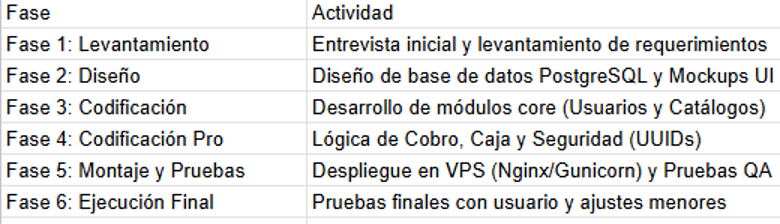
\includegraphics[width=0.8\linewidth]{imagenes/fases.png}
    \caption{Fases de desarrollo}
    \label{fig:fases_desarrollo}
\end{figure}

\section{Arquitectura del Sistema}
Para el desarrollo del sistema se implemento una  arquitectura de tres capas del sistema SIVEH, la cual garantiza una separación clara entre la interfaz, el procesamiento de datos y el almacenamiento. 

\begin{figure}[H]
    \centering
    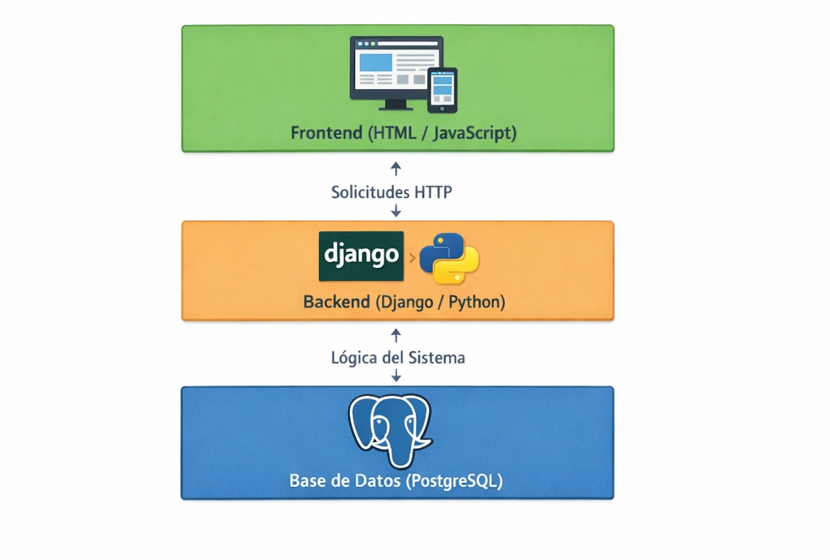
\includegraphics[width=0.8\linewidth]{imagenes/diagrama.png}
    \caption{Diagrama de bloques}
    \label{fig:Diagrama Bloques}
\end{figure}

A continuación, se detalla la función de cada componente y su interacción:

Capa de Presentación (Frontend): Es el entorno con el que interactúa el usuario final, desarrollado en HTML y JavaScript. Su función es capturar los datos de los vehículos y solicitudes administrativas para enviarlos mediante solicitudes HTTP hacia el servidor.

Capa de Lógica de Negocio (Backend): Construida sobre el framework Django y el lenguaje Python, actúa como el núcleo del sistema. Recibe las peticiones del frontend, aplica las reglas de negocio (como la validación de UUIDs o generación de folios) y coordina la comunicación con la base de datos.

Capa de Datos (Base de Datos): Utiliza el motor relacional PostgreSQL para el almacenamiento persistente. Esta capa responde a la lógica del sistema guardando o recuperando información crítica, como registros de verificaciones, inventario de hologramas y reportes financieros, asegurando la integridad y consistencia de toda la operación.

\section{Reingeniería de Procesos}
\begin{figure}[H]
    \centering
    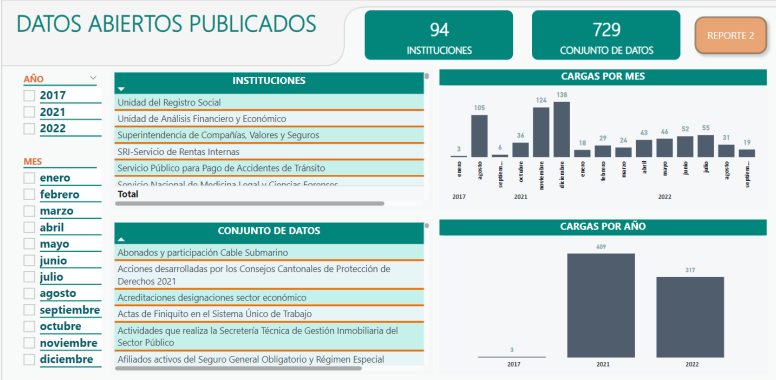
\includegraphics[width=0.8\linewidth]{imagenes/anexo2.png}
    \caption{Diagrama flujo de trabajo SIVEH}
    \label{fig:Flujo SIVEH}
\end{figure}
En la figura \ref{fig:Flujo SIVEH} se presenta la reingeniería del proceso bajo el ecosistema SIVEH. A diferencia del modelo tradicional, la arquitectura permite que la información sea capturada una sola vez y persista a lo largo de todos los módulos. Esta integración asegura que el módulo de caja y el de entrega de resultados consulten la misma instancia de la base de datos PostgreSQL, garantizando la consistencia de los datos y reduciendo el tiempo de atención al usuario final.

\section{Infraestructura de producción del sistema}
A continuación, se presenta la descripción técnica de cada componente de la infraestructura de producción del sistema SIVEH, detallando su función específica dentro del flujo de datos:

\begin{figure}[H]
    \centering
    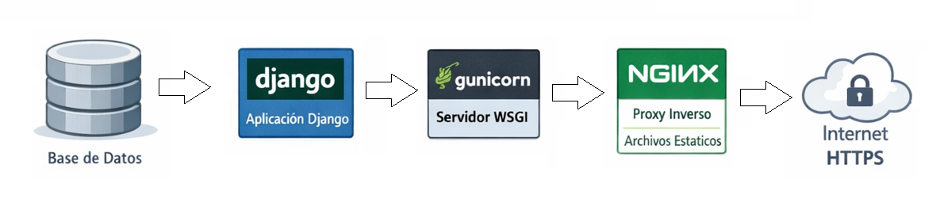
\includegraphics[width=0.8\linewidth]{imagenes/infraestructura.png}
    \caption{Diagrama inf.}
    \label{fig:infraestructura_diagrama}
\end{figure}

\subsection{Base de Datos (PostgreSQL)} 

Es la capa de persistencia donde se almacena toda la información crítica del Vericentro, incluyendo registros vehiculares, inventarios y movimientos financieros. Utiliza PostgreSQL por su robustez y cumplimiento de las propiedades ACID, garantizando que cada transacción sea íntegra y permanente. Esta capa se comunica exclusivamente con la aplicación Django a través del ORM, manteniendo los datos protegidos del acceso externo directo. Se muestra acontinuación el Modelo entidad relación de la base de datos. En el anexo se agrega a detalle las tablas que componen la base de datos ver \autoref{anexo:Tablas BD}. 


\subsection{Aplicación Django} 

Representa el cerebro del sistema o la Lógica de Negocio. Desarrollada en Python, esta capa recibe las peticiones del usuario y decide qué acciones tomar: validar un UUID, calcular una cortesía o generar un reporte contable. Django actúa como el orquestador que consulta la base de datos y renderiza la información necesaria, aplicando siempre filtros de seguridad y permisos de usuario antes de entregar cualquier respuesta.

\subsection{Servidor WSGI (Gunicorn)} 

Debido a que los servidores web tradicionales no pueden ejecutar código Python de forma nativa, se implementa Gunicorn como servidor WSGI (Web Server Gateway Interface). Su función es actuar como un puente o traductor de alto rendimiento que recibe las peticiones HTTP procesadas por el proxy y las convierte en señales que la aplicación Django puede entender y ejecutar. Es el componente encargado de gestionar múltiples procesos simultáneos para que el sistema no se ralentice.

\subsection{Proxy Inverso / Archivos Estáticos (Nginx)}

Nginx cumple una doble función vital en la arquitectura:

Proxy Inverso: Actúa como un escudo y receptor de tráfico; recibe las peticiones de internet y las distribuye eficientemente al servidor WSGI, protegiendo la identidad interna del servidor de aplicaciones.

Gestión de Archivos Estáticos: Se encarga de servir directamente los recursos visuales (CSS, JavaScript e imágenes) sin pasar por Django. Esto libera de carga al backend y acelera significativamente la velocidad de carga de la interfaz de usuario.

\subsection{Internet HTTPS}

Representa el punto de contacto con el usuario final. Toda la comunicación entre el navegador del cliente y el servidor se realiza a través del protocolo HTTPS, lo que significa que los datos viajan cifrados mediante certificados SSL/TLS. Esto garantiza la confidencialidad de la información sensible (como folios de pago y datos de propietarios) y asegura la identidad del servidor de Hostinger ante cualquier intento de interceptación en la red.\\

\section{Codificación e Implementación}

La implementación del sistema SIVEH se estructuró bajo el patrón arquitectónico Modelo-Vista-Template (MVT) de Django, lo que permitió una separación estricta entre la persistencia de datos, la lógica de control y la interfaz de usuario. La orquestación del sistema se centraliza en el archivo \verb|urls.py| para el enrutamiento de peticiones, mientras que la inteligencia operativa reside en  \verb|views.py|.

En esta etapa de codificación, se priorizó la seguridad y la integridad de los datos mediante el uso de Identificadores Únicos Universales (UUIDs) y validaciones a nivel de servidor que previenen la duplicidad de folios. Asimismo, se integraron bibliotecas especializadas como Openpyxl para automatizar la generación de reportes contables en formato  \verb|.xlsx|, y se implementaron selectores dinámicos en las plantillas HTML para minimizar errores de captura manual.

A continuación, se analizan los fragmentos de código más representativos de la lógica del sistema, detallando el funcionamiento de las vistas que gestionan los procesos críticos del verificentro:

\subsection{Vista: reporte\_ventas\_view (Módulo de Administración)}

Esta sección del código corresponde a una vista desarrollada en el framework Django, cuya finalidad es generar reportes financieros dinámicos dentro del sistema SIVEH.

A nivel de programación, esta vista fue construida utilizando el patrón Modelo-Vista-Template (MVT) propio de Django, donde la vista actúa como intermediaria entre la interfaz del usuario y la base de datos. El flujo inicia cuando el administrador envía una solicitud HTTP (generalmente mediante un formulario con filtros de fecha y tipo de pago). El sistema recibe estos parámetros y ejecuta consultas a través del ORM de Django, evitando el uso directo de SQL.

El código realiza principalmente las siguientes acciones:

\begin{itemize}
    \item Valida que el usuario tenga una sesión activa y permisos administrativos, garantizando la seguridad del sistema. 
    \item Filtra los registros de verificaciones y ventas en función de los parámetros proporcionados. 
    \item Realiza operaciones de agregación (sumatorias) directamente en la base de datos, optimizando el rendimiento. 
    \item Organiza los resultados en estructuras de datos que posteriormente son renderizadas en la interfaz. 
\end{itemize}
Adicionalmente, se implementa una funcionalidad de exportación a Excel, la cual se programó utilizando librerías de Python que permiten generar archivos en formato .xlsx. Esta característica facilita la portabilidad de la información y su uso en procesos contables externos.

En resumen, esta vista fue diseñada para automatizar el análisis financiero del verificentro, reduciendo errores humanos y tiempos de procesamiento.\\
\begin{figure}[H]
    \centering
    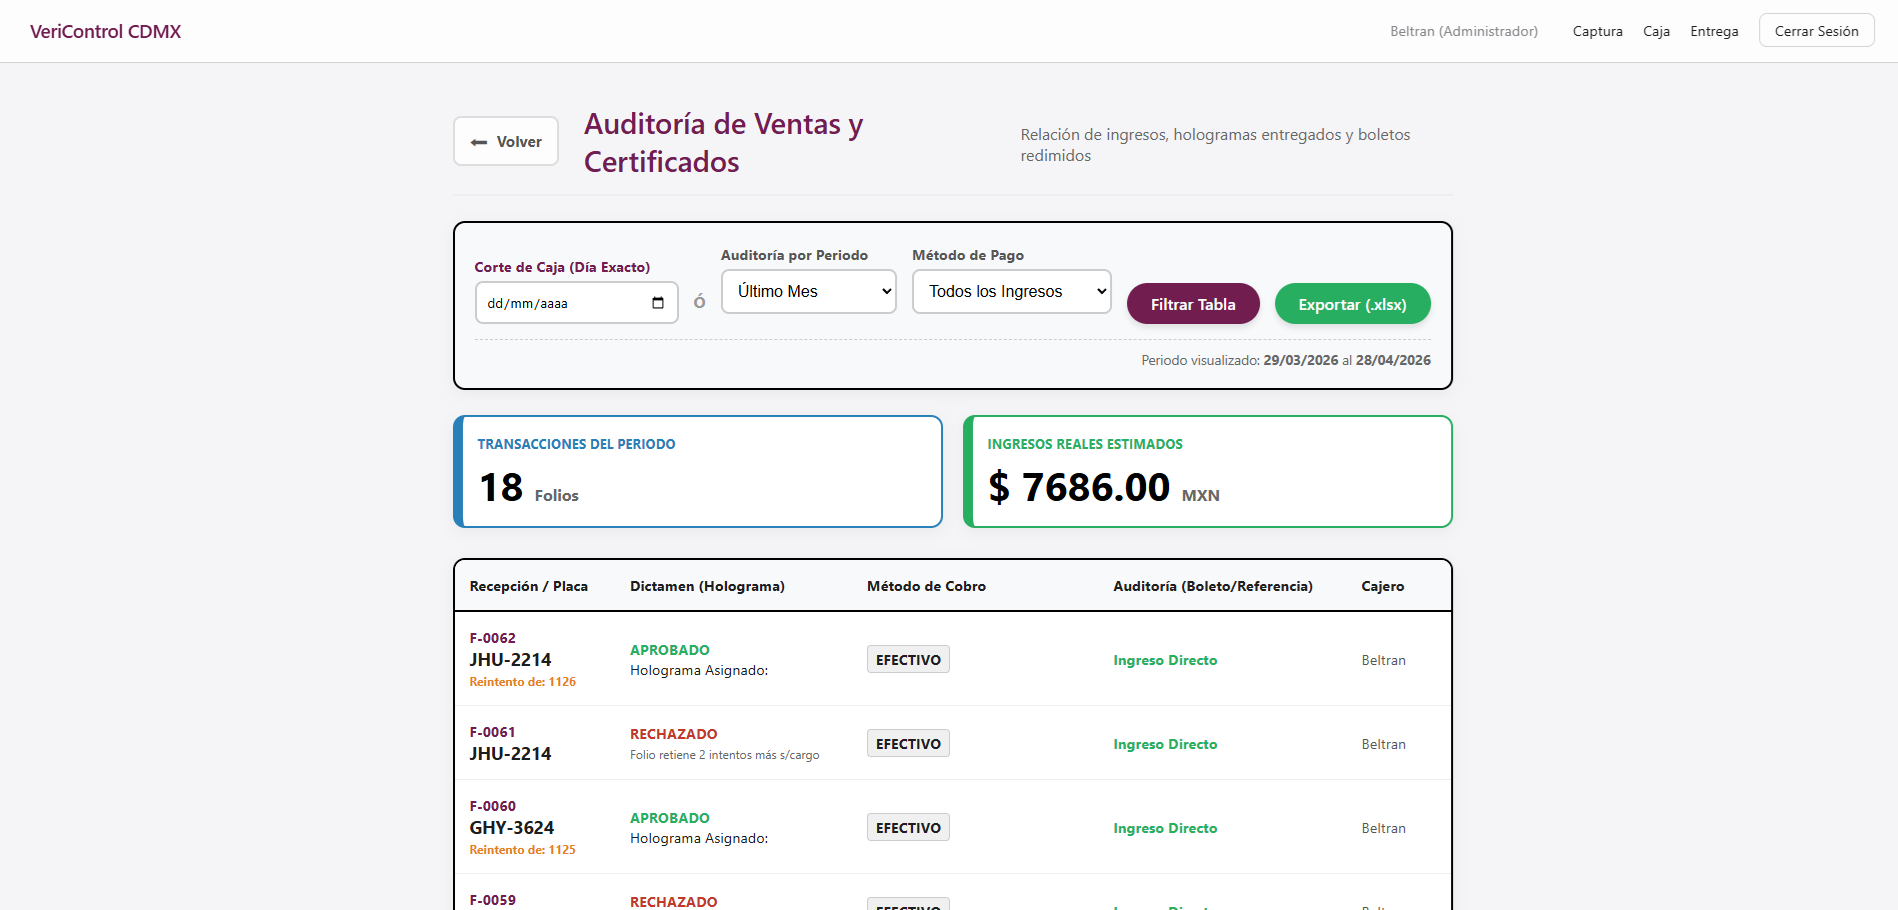
\includegraphics[width=0.8\linewidth]{imagenes/Reporte de ventas.png}
    \caption{Captura }
    \label{fig:Reporte Ven V}
\end{figure}
\begin{figure}[H]
    \centering
    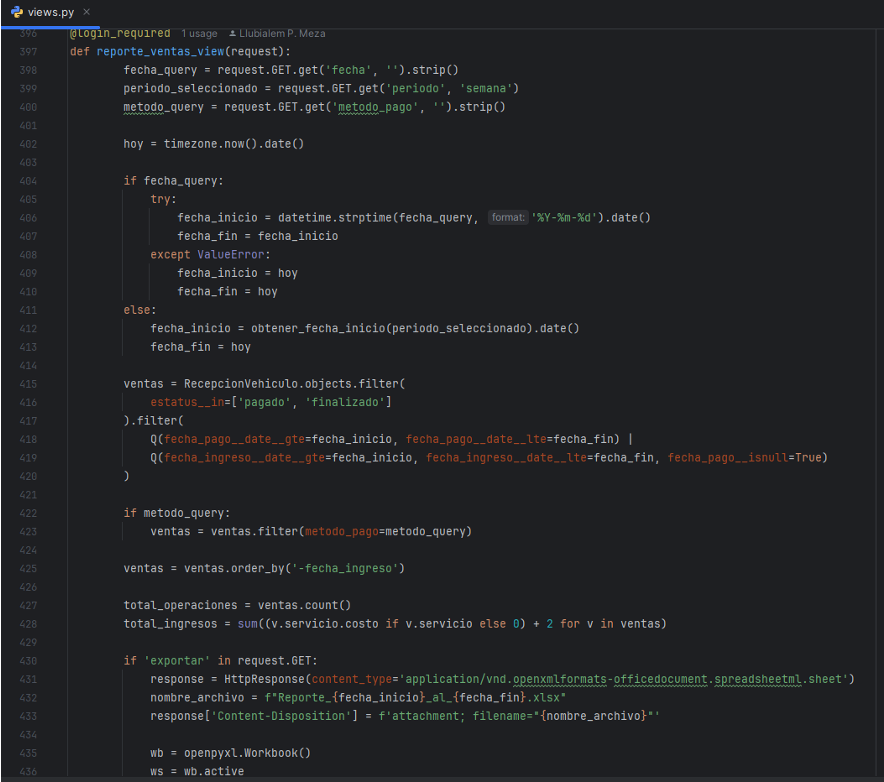
\includegraphics[width=0.8\linewidth]{imagenes/desarrollo1.1.png}
    \caption{Reporte Ventas View}
    \label{fig:reporte_ventas_view}
\end{figure}

\subsection{Vista: captura\_view (Módulo de Recepción)}

Esta vista representa uno de los componentes más críticos del sistema, ya que es responsable del registro y validación de los vehículos que ingresan al proceso de verificación.

Desde el punto de vista técnico, el código fue desarrollado bajo principios de Programación Orientada a Objetos (POO), donde cada entidad (vehículo, taller, servicio) se modela como un objeto dentro del sistema. La vista interactúa con estos modelos mediante el ORM de Django.

El funcionamiento del código se basa en:

\begin{itemize}
    \item Recepción de datos desde formularios en el frontend. 
    \item Validación de campos obligatorios como placas, número de serie y tipo de servicio. 
    \item Verificación de reglas de negocio, como: 
    \begin{itemize}
        \item Evitar registros duplicados en el mismo periodo. 
        \item Validar si el vehículo tiene rechazos previos. 
        \item Determinar si aplica una justificación (multa o reemplazo). 
    \end{itemize}
\end{itemize}
El sistema también implementa restricciones que impiden guardar información incompleta o inconsistente, lo cual se logra mediante validaciones tanto en el frontend (JavaScript) como en el backend (Python).

Otro aspecto importante es el control de permisos, donde solo usuarios autorizados pueden modificar registros existentes. Esto se implementa mediante decoradores de Django y validaciones de sesión.

En términos de desarrollo, esta vista fue programada con enfoque en la integridad de datos, asegurando que toda la información capturada cumpla con las reglas operativas del verificentro antes de almacenarse en la base de datos.
\\
\begin{figure}[H]
    \centering
    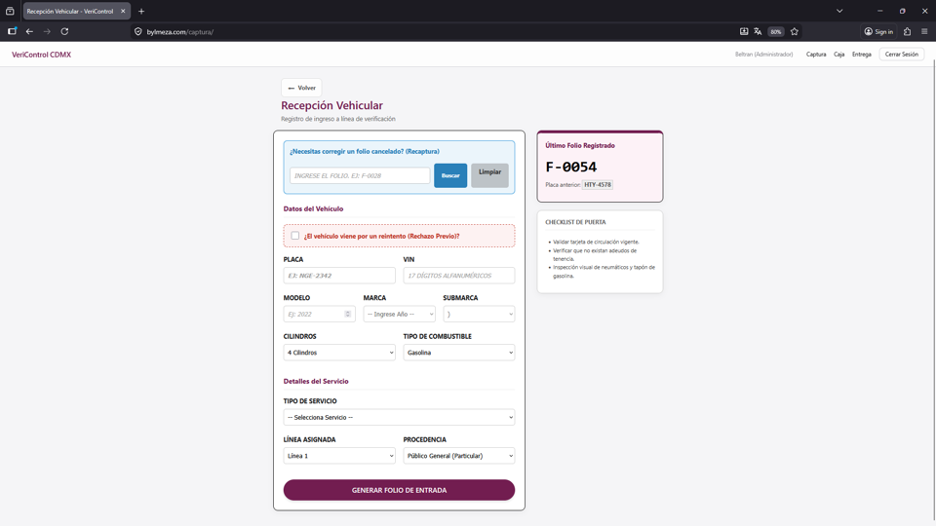
\includegraphics[width=0.8\linewidth]{imagenes/pruebas2.png}
    \caption{Captura }
    \label{fig:Captura V}
\end{figure}

\begin{figure}[H]
    \centering
    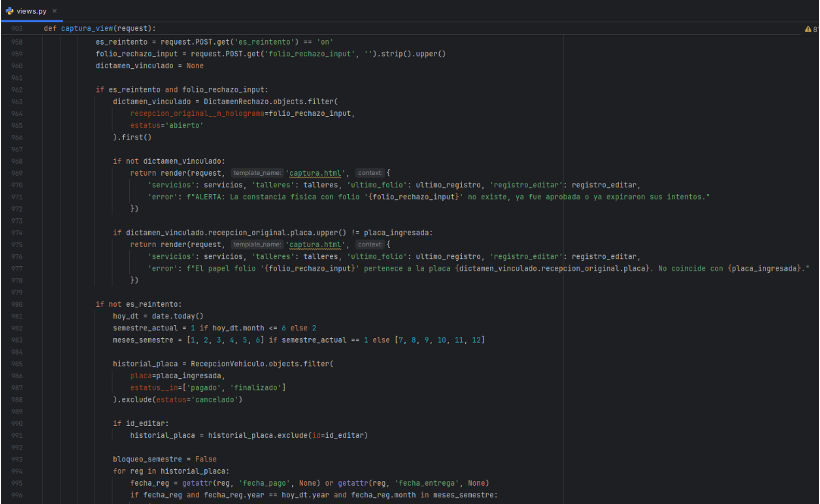
\includegraphics[width=0.8\linewidth]{imagenes/desarrollo1.3.png}
    \caption{Vista Captura-view}
    \label{fig:captura_view_1_3}
\end{figure}

\begin{figure}[H]
    \centering
    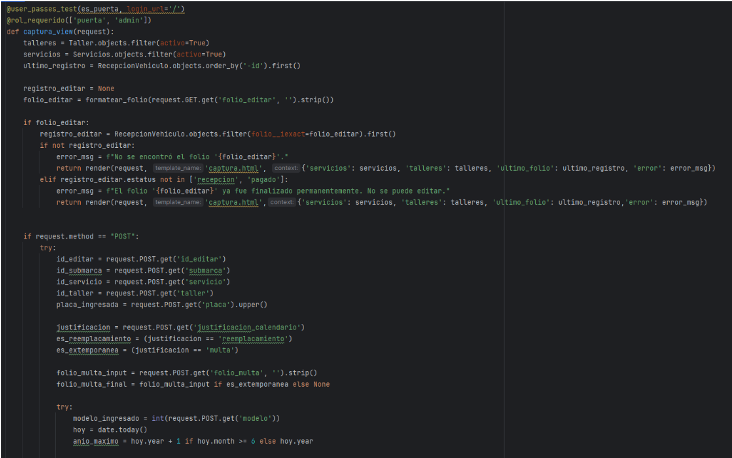
\includegraphics[width=0.8\linewidth]{imagenes/desarrollo1.2.png}
    \caption{Vista Captura-view 2}
    \label{fig:captura_view_1_2}
\end{figure}


\subsection{Vista: caja\_view (Módulo de Cobro)}

El código de esta vista gestiona todo el flujo de pagos dentro del sistema, integrando múltiples métodos de cobro y validaciones comerciales.

A nivel técnico, esta vista se encarga de procesar transacciones, por lo que fue diseñada considerando principios de atomicidad (propiedad ACID de la base de datos). Esto significa que cada operación de pago se ejecuta completamente o no se ejecuta, evitando inconsistencias.

El proceso programado en el código incluye:

\begin{itemize}
    \item Recepción del folio del vehículo previamente registrado. 
    \item Validación de métodos de pago (efectivo, tarjeta, crédito, prepago o cortesía). 
    \item Verificación de boletos de prepago mediante consultas a la base de datos. 
    \item Validación de correspondencia entre el boleto y el taller, evitando fraudes o errores administrativos. 
\end{itemize}
Una funcionalidad destacada es el programa de lealtad, el cual fue implementado mediante lógica condicional en el backend. El sistema lleva un conteo automático de servicios realizados por cliente y, al alcanzar un umbral (ocho servicios), genera un boleto de cortesía.

Finalmente, el código registra:

\begin{itemize}
    \item El usuario (cajero) que realizó la operación. 
    \item El método de pago utilizado. 
    \item La transacción en la base de datos. 
\end{itemize}
Posteriormente, redirige al módulo de impresión de tickets.

Esta vista fue programada para garantizar rapidez en la atención al cliente y precisión en el control financiero.
\\
\begin{figure}[H]
    \centering
    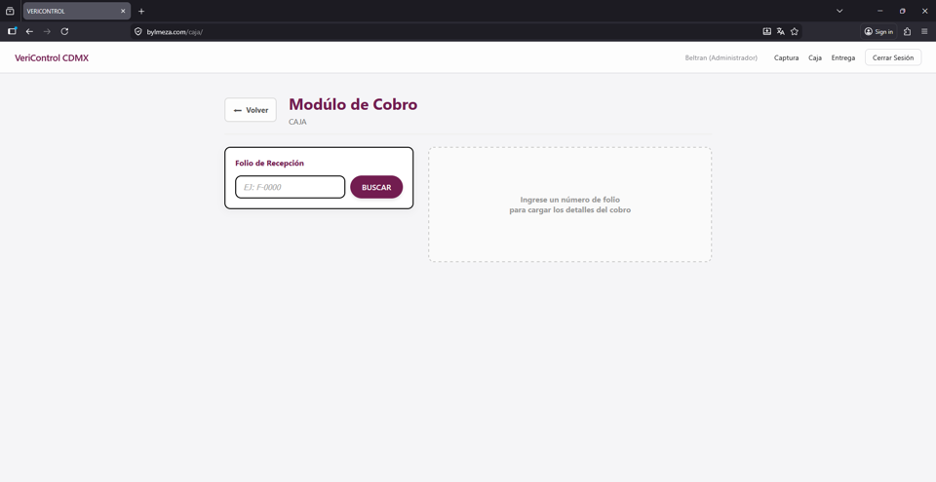
\includegraphics[width=0.8\linewidth]{imagenes/prueba5.png}
    \caption{Caja modulo cobro de servicio }
    \label{fig:caja_modulo_cobro}
\end{figure}

\begin{figure}[H]
    \centering
    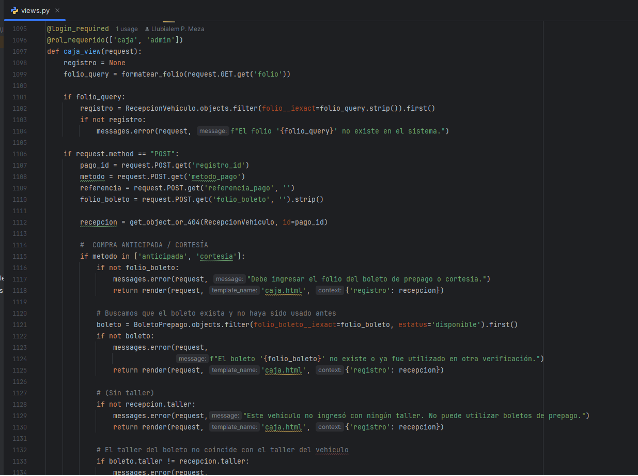
\includegraphics[width=0.8\linewidth]{imagenes/desarrollo1.4.png}
    \caption{Vista caja-view}
    \label{fig:caja_view_1_4}
\end{figure}

\begin{figure}[H]
    \centering
    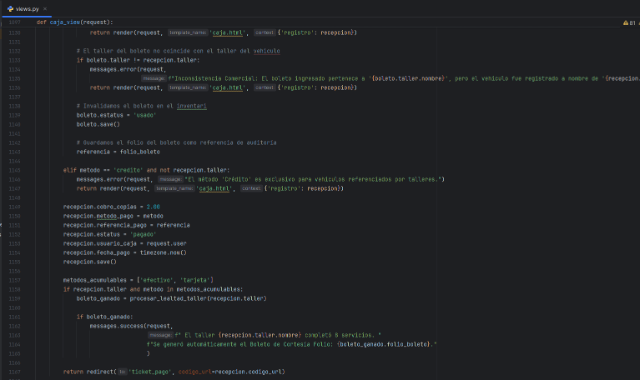
\includegraphics[width=0.8\linewidth]{imagenes/desarrollo1.5.png}
    \caption{Vista caja-view pt.2}
    \label{fig:caja_view_1_5}
\end{figure}


\subsection{Vista: entrega\_view (Módulo de Entrega de Resultados)}

Esta vista corresponde a la etapa final del proceso de verificación vehicular, donde se entrega el resultado y el holograma correspondiente.

El código implementa una lógica automatizada que determina el tipo de holograma basado en características del vehículo, como:

\begin{itemize}
    \item Año modelo 
    \item Tipo de combustible 
    \item Resultado de la verificación (aprobado o rechazado) 
\end{itemize}
A nivel técnico, el flujo del sistema es el siguiente:

\begin{itemize}
    \item Validación de que el pago haya sido realizado previamente (integración con módulo de caja). 
    \item Consulta del inventario de hologramas disponible en la base de datos. 
    \item Asignación automática del siguiente folio físico disponible. 
    \item Registro del dictamen técnico y del usuario responsable. 
\end{itemize}
El sistema también incluye controles de seguridad avanzados:

\begin{itemize}
    \item Restricción de cancelación de hologramas a usuarios con rol administrativo. 
    \item Protección de registros históricos para evitar alteraciones indebidas. 
    \item Trazabilidad completa de cada holograma asignado. 
\end{itemize}
La programación de esta vista se realizó priorizando la sincronización entre módulos y la reducción de errores humanos, utilizando consultas eficientes y validaciones en tiempo real.
\\
\begin{figure}[H]
    \centering
    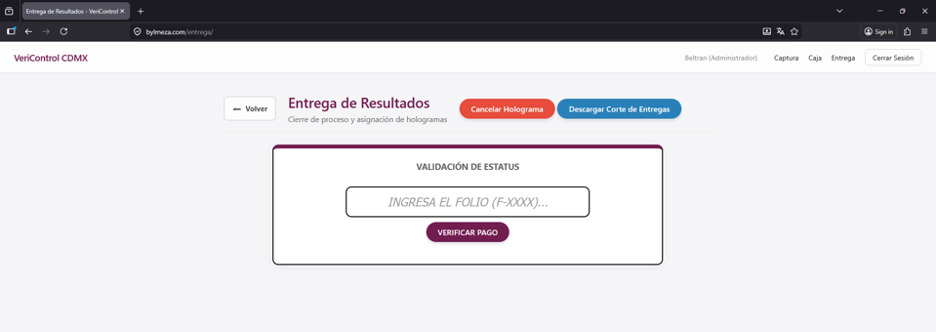
\includegraphics[width=0.8\linewidth]{imagenes/prueba11.png}
    \caption{Entrega de resultados}
    \label{fig:entrega_resultados}
\end{figure}

\begin{figure}[H]
    \centering
    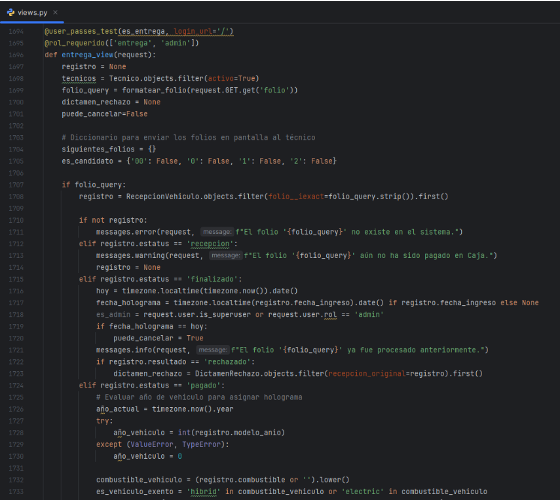
\includegraphics[width=0.8\linewidth]{imagenes/desarrollo1.6.png}
    \caption{Vista entrega view}
    \label{fig:entrega_view_1_6}
\end{figure}

\begin{figure}[H]
    \centering
    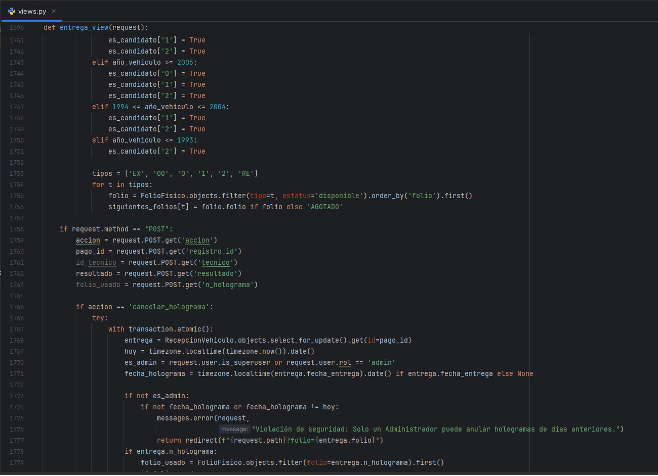
\includegraphics[width=0.8\linewidth]{imagenes/desarrollo1.7.png}
    \caption{Vista entrega view}
    \label{fig:entrega_view_1_7}
\end{figure}


\textbf{Debido a la extensión del proyecto, en este apartado se exponen solo los componentes clave del código. La versión íntegra y funcional del software está disponible para su consulta en el repositorio de GitHub referenciado en el \ref{anexo:github}}
\\

\section{Pruebas}
El objetivo de esta seccion es documentar el proceso de verificación y validación del sistema SIVEH, asegurando que cada componente cumpla con los requisitos técnicos y operativos establecidos. Se aplicó una estrategia de pruebas multinivel para garantizar la estabilidad, seguridad e integridad de los datos en el entorno de producción.
\subsection{Pruebas Unitarias}
Las pruebas unitarias se enfocaron en la verificación de funciones y métodos individuales de forma aislada. En el ecosistema Django, se utilizaron las herramientas nativas de \verb|django.test| para validar la lógica crítica sin depender de factores externos.

\begin{itemize}
    \item \textbf{Validación de UUIDs:} Se comprobó que cada registro generado contara con un identificador único y que el sistema rechazara cualquier intento de acceso mediante ID secuenciales.
    \begin{figure}[H]
    \centering
    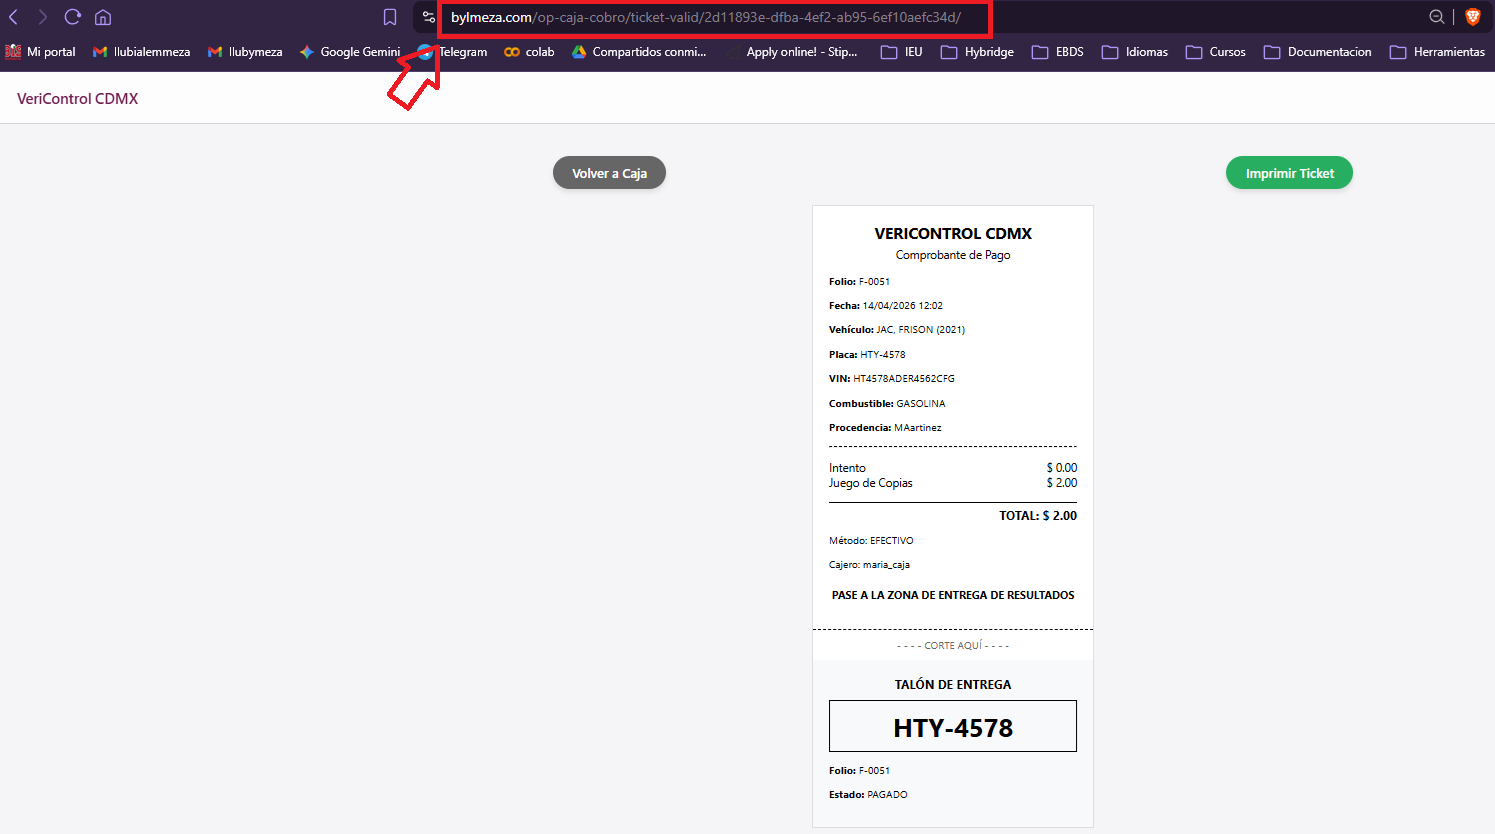
\includegraphics[width=0.8\linewidth]{imagenes/validacion UUID.png}
    \caption{Validacion de UUIDs}
    \label{fig:validacio uuid}
\end{figure}
\begin{figure}[H]
    \centering
    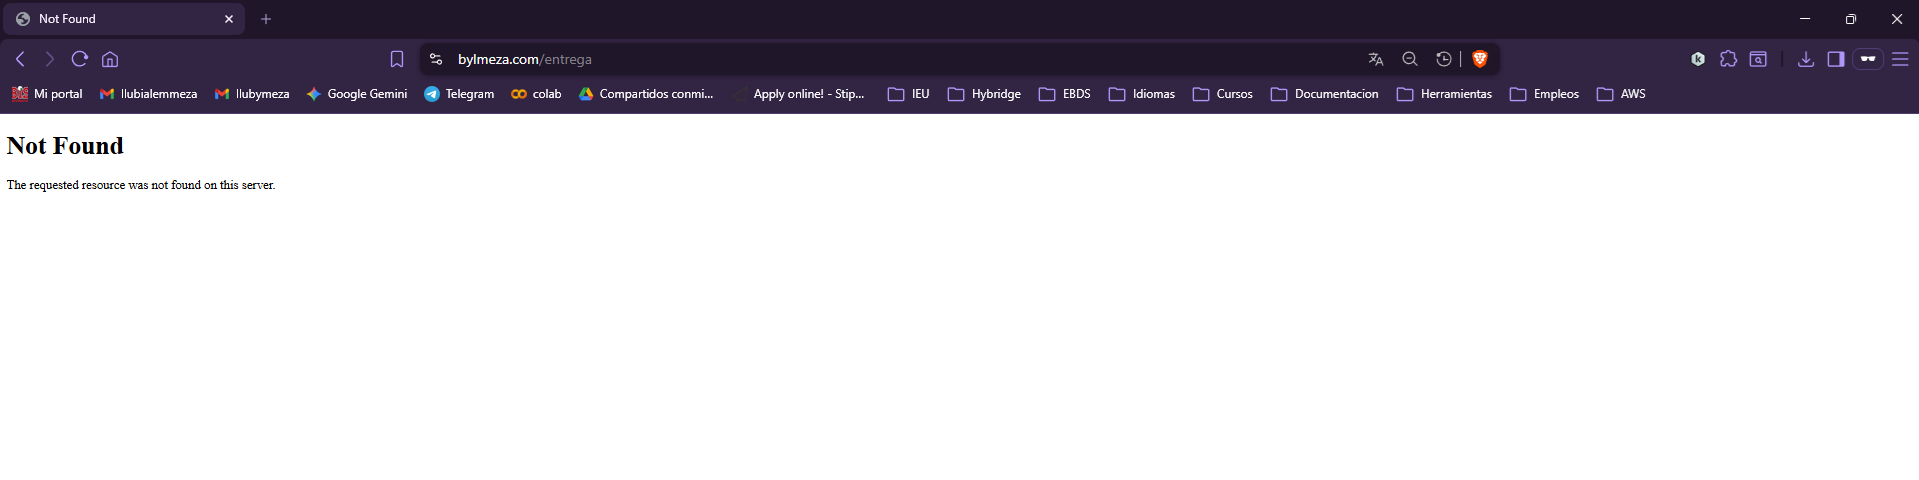
\includegraphics[width=0.8\linewidth]{imagenes/validacion UUID2.png}
    \caption{Intento con ID simple}
    \label{fig:validacion uidd2}
\end{figure}
Las Figuras \ref{fig:validacio uuid} y \ref{fig:validacion uidd2} evidencian la implementación de UUIDs; el sistema rechaza peticiones mediante identificadores secuenciales, protegiendo la información de intentos de enumeración de recursos.

    \item \textbf{Cálculo de Costos y Cortesías:} Se ejecutaron casos de prueba para asegurar que la lógica de 'octava verificación gratuita' se active exactamente al cumplir los criterios, evitando errores en el saldo del cajero.
    \item \textbf{Reglas de Negocio en Modelos:} Se validaron las restricciones de los campos en PostgreSQL, como la imposibilidad de registrar una placa duplicada en el mismo periodo semestral.
\end{itemize}

\subsection{Pruebas de Integración}
Estas pruebas evaluaron la comunicación efectiva entre los diferentes módulos del sistema y las capas de la arquitectura. Se puso especial énfasis en el flujo de datos desde la interfaz hasta la persistencia final.

\begin{itemize}
    \item \textbf{Interacción ORM-Base de Datos:} Se verificó que las consultas complejas realizadas mediante el ORM de Django se tradujeran en transacciones SQL eficientes en PostgreSQL, manteniendo la integridad referencial.
    \item \textbf{Comunicación WSGI:} Se realizaron pruebas de comunicación entre Gunicorn y la aplicación Django para asegurar que las peticiones HTTP fueran procesadas y respondidas sin pérdida de cabeceras de seguridad.
    \item \textbf{Gestión de Archivos Estáticos:} Se validó que Nginx sirviera correctamente los recursos CSS y JavaScript, permitiendo que la lógica del frontend (selectores en cascada) operara en sincronía con los datos del backend.
\end{itemize}

\subsection{Pruebas Funcionales}
Las pruebas funcionales validaron que el sistema respondiera correctamente a las necesidades del usuario final mediante la simulación de escenarios reales.

\begin{itemize}
    \item \textbf{Ciclo Completo de Verificación:} Se simuló el flujo desde la captura inicial del vehículo, el paso por el módulo de caja para el cobro del servicio, hasta la asignación final del holograma.
    \item \textbf{Generación de Reportes:} Se verificó que el módulo de administración generara archivos Excel (.xlsx) con datos precisos, filtrando correctamente por fechas y estados de pago, tal como se especificó en los requerimientos.
    \begin{figure}[H]
    \centering
    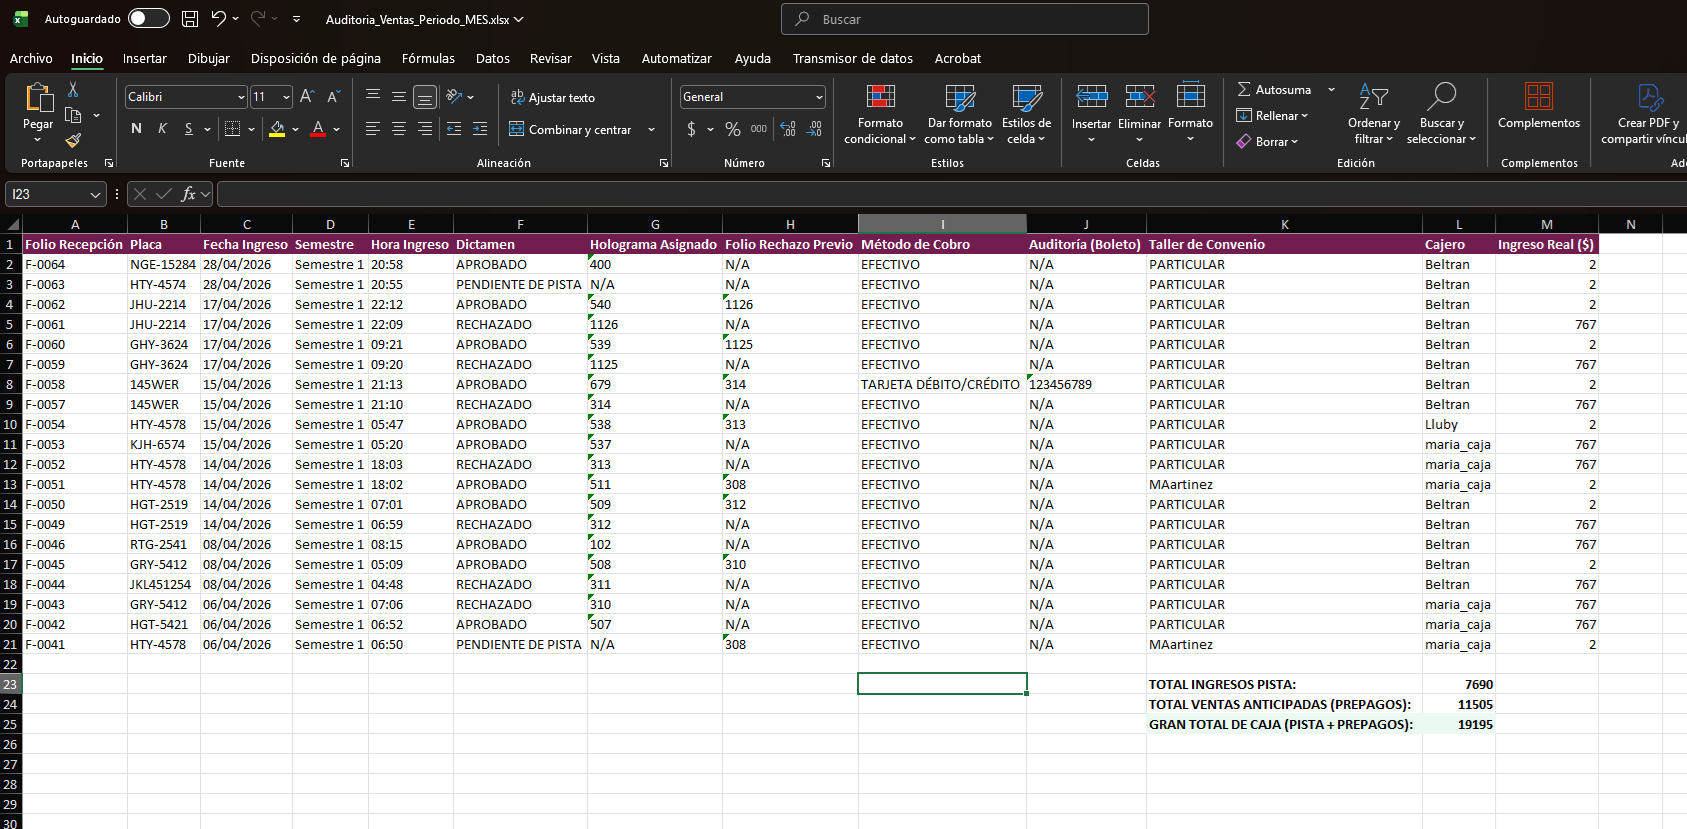
\includegraphics[width=0.8\linewidth]{imagenes/ReporteExcel.png}
    \caption{Reporte generado del ultimo mes}
    \label{fig:Reporte Excel}
\end{figure}
En la Fig.Fig.\ref{fig:Reporte Excel} se muestra el reporte generado por el sistema en formato .xlsx, validando que la integración con la biblioteca Openpyxl extrae correctamente los montos y fechas de la base de datos PostgreSQL.
\end{itemize}

\subsection{Pruebas de Rendimiento}
Dada la naturaleza crítica del tiempo de atención en un verificentro, se midió la respuesta del sistema bajo condiciones de carga en el servidor de producción.

\begin{itemize}
    \item \textbf{Concurrencia:} Se monitoreó el comportamiento del servidor ante múltiples peticiones simultáneas en los módulos de captura y caja, observando que el uso de memoria se mantuvo estable gracias a la gestión de procesos de Gunicorn.
    
\begin{figure}[H]
    \centering
    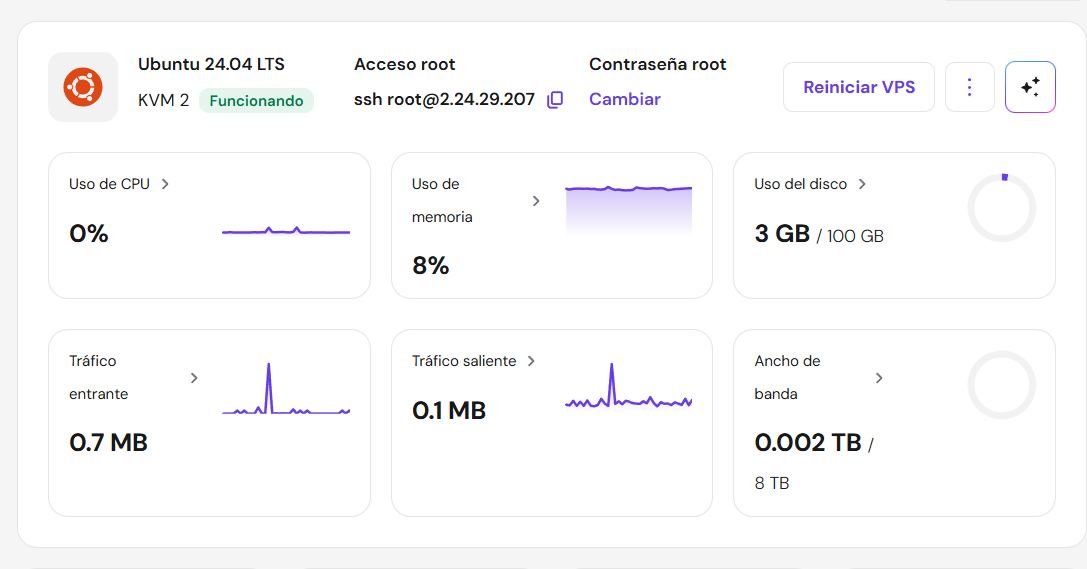
\includegraphics[width=0.8\linewidth]{imagenes/rendimiento.png}
    \caption{Rendimiento VPS}
    \label{fig:Rendimiento}
\end{figure}

    \item \textbf{Tiempos de Respuesta:} Se registraron tiempos de respuesta promedio inferiores a 200ms en consultas locales y menos de 1s en la generación de reportes complejos, cumpliendo con los estándares de eficiencia esperados para una aplicación web moderna.
\end{itemize}



\subsection{Pruebas de Usuario}
Finalmente, el sistema fue evaluado por el personal operativo del verificentro. Estas pruebas se integraron de manera incremental durante las revisiones de los martes, de acuerdo con la metodología Scrum.

\begin{itemize}
    \item \textbf{Usabilidad:} Los usuarios confirmaron que la interfaz reduce la fatiga visual durante jornadas largas de trabajo.
    \item \textbf{Experiencia de Usuario:} Se validó que la reducción de pasos manuales y la eliminación de hojas de cálculo externas facilitan el aprendizaje del sistema para nuevos empleados.
    \item \textbf{Aceptación Final:} El personal administrativo validó la precisión de los cierres de caja automáticos, otorgando el visto bueno para la transición completa al ecosistema SIVEH.
\end{itemize}


\chapter{Resultados}

En este capítulo se presentan los resultados obtenidos tras la implementación y puesta en marcha del sistema SIVEH en el entorno operativo del verificentro. La evaluación se fundamenta en un análisis mixto que combina métricas cuantitativas de rendimiento y la percepción cualitativa de los usuarios finales recolectada mediante cuestionarios estructurados ver \autoref{anexo:Cuestionarios}.

\section{Optimización de la Eficiencia Operativa}

El impacto más significativo del sistema se observa en la drástica reducción de los tiempos de procesamiento. Al centralizar la información en una arquitectura web, se eliminó la latencia provocada por la consulta de múltiples archivos de Excel y bitácoras físicas.

\begin{figure}[H]
    \centering
    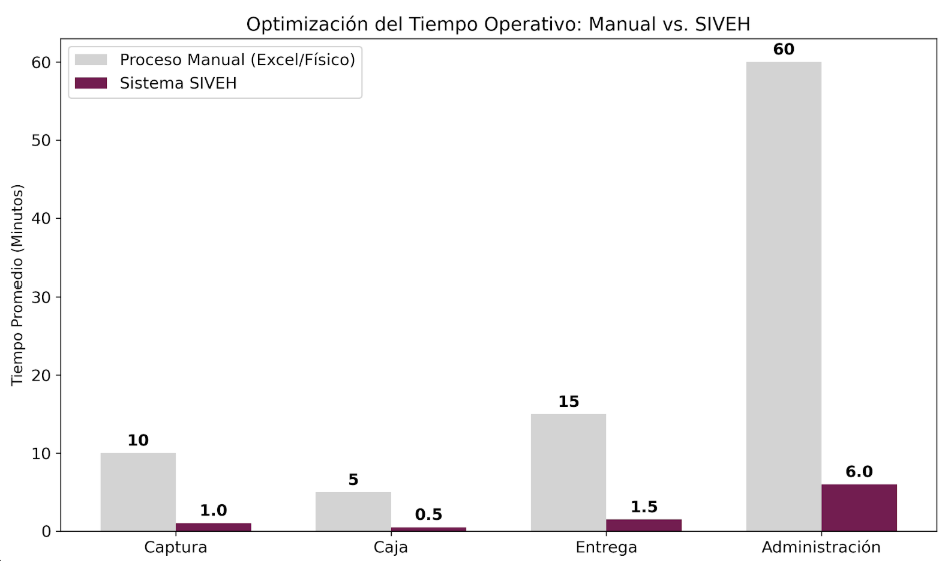
\includegraphics[width=0.7\linewidth]{imagenes/grafico tiempo de operacion.png}
    \caption{Comparativa de tiempos promedio de operación por módulo (en minutos).}
    \label{fig:tiempos_minutos}
\end{figure}

Como se aprecia en la Fig. \ref{fig:tiempos_minutos}, se logró una optimización del 90\% en las tareas críticas. El área administrativa redujo su carga de conciliación de 60 a solo 6 minutos. Los usuarios de caja y captura validaron esta métrica mediante sus testimonios, destacando que \textit{"antes se pasaban horas cuadrando el Excel con lo físico, y ahora con los reportes automáticos todo sale a la primera"}.

\section{Integridad y Confiabilidad de la Información}

La transición de un sistema basado en hojas de cálculo a un motor relacional PostgreSQL permitió blindar la integridad de los datos. Se evaluó la precisión de la información contrastando los registros históricos con los generados por SIVEH.

\begin{figure}[H]
    \centering
    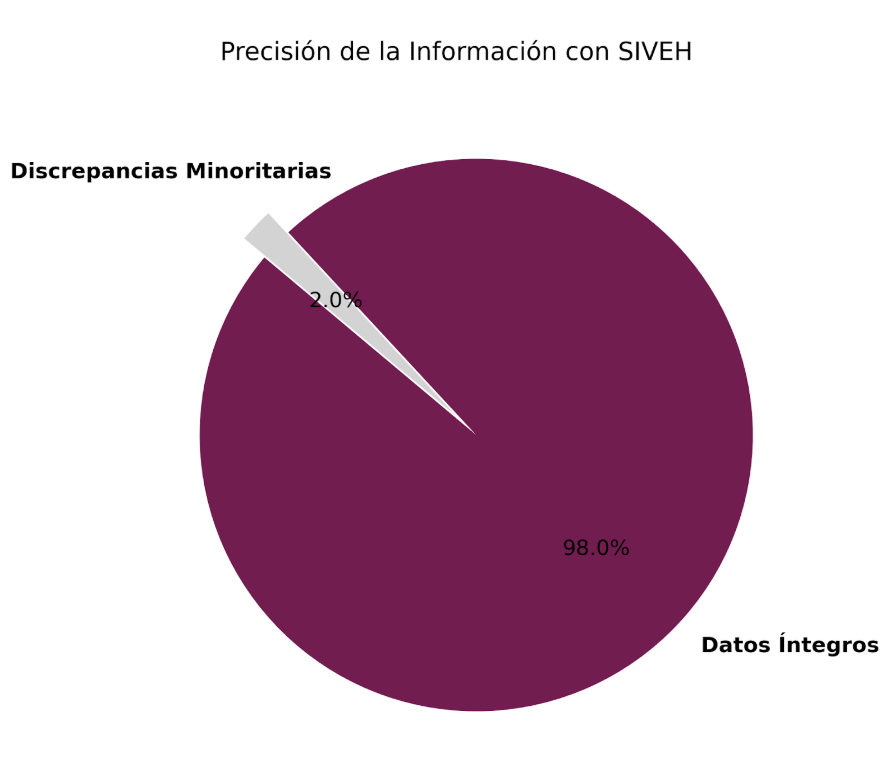
\includegraphics[width=0.7\linewidth]{imagenes/grafico precision.png}
    \caption{Análisis de precisión e integridad de los datos en el ecosistema SIVEH.}
    \label{fig:precision_datos}
\end{figure}

La Fig. \ref{fig:precision_datos} ilustra que el 98\% de la información procesada se mantiene con total integridad. El 2\% de discrepancias detectadas se asocia a la depuración de datos erróneos provenientes del sistema anterior. Esta robustez técnica fue confirmada por el área de entrega de resultados, quienes reportaron una disminución total en los errores de asignación de hologramas, señalando que \textit{"el hecho de que el folio esté amarrado digitalmente al vehículo otorga seguridad al operador y al cliente"}.

\section{Evaluación de la Experiencia de Usuario (UX/UI)}

La aceptación del sistema por parte del personal operativo es un indicador clave del éxito del proyecto. Se evaluaron cuatro pilares fundamentales de la interfaz: facilidad de uso, diseño visual, confianza en los datos y velocidad de respuesta.

\begin{figure}[H]
    \centering
    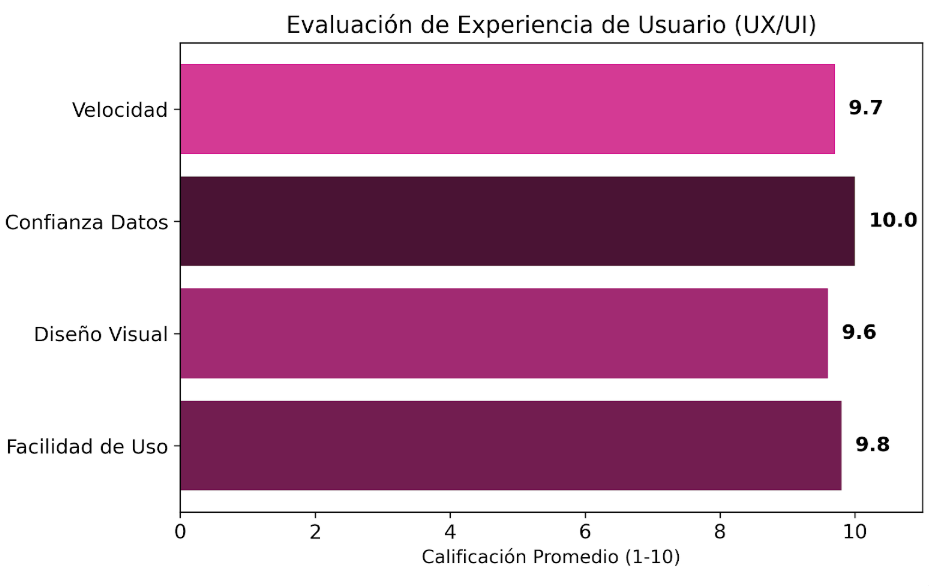
\includegraphics[width=0.7\linewidth]{imagenes/grafico UX.png}
    \caption{Métricas de aceptabilidad y ergonomía de la interfaz de usuario.}
    \label{fig:satisfaccion_ux}
\end{figure}

Los resultados presentados en la Fig. \ref{fig:satisfaccion_ux} muestran una calificación promedio de 9.8/10 en amigabilidad. Los operadores de captura enfatizaron la ergonomía del diseño, mencionando que \textit{"la paleta de colores no cansa la vista durante jornadas prolongadas"}. Asimismo, la disposición lógica de los menús permitió que el sistema fuera intuitivo, eliminando la necesidad de manuales extensos y facilitando la fluidez del trabajo mediante el uso de comandos de teclado.

\section{Impacto en la Gestión Administrativa}

Finalmente, el módulo administrativo demostró ser una herramienta estratégica para la toma de decisiones. La implementación de alertas de inventario en tiempo real y la automatización de los cortes de caja permitieron al administrador reducir a la mitad el tiempo dedicado a la supervisión contable.

Los usuarios de caja destacaron la claridad de los reportes generados: \textit{"Ya no tengo que estar rezando para que no me haya faltado un ticket; el sistema desglosa todo por tipo de pago y el total sale exacto"}. Este nivel de precisión asegura una transparencia total en las finanzas del verificentro y una logística eficiente en la solicitud de nuevos hologramas a la bóveda central.
\chapter{Conclusiones}

La implementación de la Plataforma de Análisis Estadístico Académico resolvió de manera definitiva la fragmentación y dispersión de la información escolar en la Universidad Politécnica de Texcoco. El sistema transformó por completo la forma en que se manejan los datos dentro de la institución, pasando de un proceso manual en hojas de cálculo que tomaba días a una plataforma rápida y segura que entrega resultados claros en corto tiempo. Esto no solo agiliza el trabajo diario en la oficina académica, sino que brinda a los directivos y coordinadores información real y oportuna para entender mejor el avance de los estudiantes, prevenir la deserción y tomar decisiones que realmente beneficien a la comunidad universitaria.

Para nosotros, desarrollar este proyecto fue el mayor reto de nuestra carrera y una experiencia que nos cambió como futuros ingenieros. Salir de los ejercicios del aula y enfrentarnos a un problema real nos enseñó que programar va mucho más allá de escribir código; implicó escuchar a los usuarios, entender sus problemas del día a día, limpiar información compleja y buscar soluciones prácticas cuando las cosas no salían al primer intento.

Más allá del aprendizaje técnico, este proyecto nos deja la satisfacción de haber creado algo útil y con un impacto positivo para nuestra propia universidad. Nos demostró de lo que somos capaces cuando unimos esfuerzos, dedicación y compromiso. Concluir esta etapa nos llena de orgullo y nos da la seguridad y motivación necesarias para dar el siguiente paso y enfrentar con entusiasmo nuestro camino en el mundo profesional.

\newpage
\cleardoublepage
\addcontentsline{toc}{chapter}{ANEXOS}
\section*{ANEXOS}

\appendix
\renewcommand{\thesection}{Anexo \Alph{section}} 
\addtocontents{toc}{\protect\fixAnexoToc}

\section{Repositorio GitHub}
\label{anexo:github}

\begin{figure}[htbp]
    \centering
    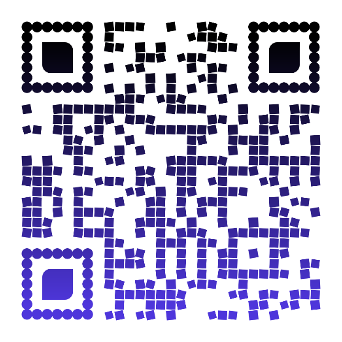
\includegraphics[width=0.8\linewidth]{imagenes/Repositorio.png}
    \caption{Repositorio de Github}
    \label{fig:repo_qr}
\end{figure}

\section{Cuestionario a usuarios}
\label{anexo:Cuestionarios}
Se realizaron cuestionarios a los usuarios del sistema, los cuestionarios fueron adaptados a el area correspondiente de cada usuario.
\subsection{Cuestionario a Administradores}
 \begin{enumerate}
     \item ¿Qué tan eficiente considera la generación de reportes administrativos en comparación con el manejo anterior en Excel?
    \item ¿El sistema le permite identificar con claridad las discrepancias en el inventario de hologramas en tiempo real?
    \item ¿Cómo califica la utilidad de las alertas de la bóveda para la planeación de la logística de hologramas?
    \item ¿Considera que el módulo administrativo facilita el seguimiento contable de los movimientos diarios del verificentro?
    \item ¿Qué funcionalidad adicional de supervisión agregaría para mejorar el control de las operaciones?
\end{enumerate}

\subsection{Cuestionario a Usuarios de Captura}
\begin{enumerate}
    \item ¿Qué tan intuitiva resulta la interfaz de captura comparada con el uso de hojas de cálculo de Excel?
    \item ¿El sistema le ayuda a prevenir errores de dedo mediante validaciones automáticas durante el ingreso de datos?
    \item ¿Considera que el diseño de las vistas de captura es ergonómico para jornadas de trabajo prolongadas?
    \item ¿Qué proceso manual que aún realiza cree que debería integrarse totalmente a esta vista?
\end{enumerate}

\subsection{Cuestionario a usuarios modulo Caja}
\begin{enumerate}
    \item ¿Cómo ha cambiado el tiempo de captura de información interna en el sistema comparado con el proceso anterior?
    \item ¿El flujo de recepción de documentos en "puerta" se integra de manera fluida con el registro en el módulo de caja?
    \item ¿Qué tan claros son los reportes de corte de caja que genera el sistema al final del turno?
    \item ¿Ha experimentado errores en la validación de datos durante la captura que el sistema no haya detectado?
    \item ¿La interfaz le permite gestionar los pagos de forma rápida para evitar cuellos de botella en la atención?
\end{enumerate}

\subsection{Cuestionario usuarios modulo Entrega de resultados}
\begin{enumerate}
    \item ¿Cómo califica la efectividad de las alertas al momento de preparar la entrega del resultado y el holograma?
    \item ¿El proceso de generación del reporte final de resultados es más ágil que cuando se realizaba manualmente?
    \item ¿Ha notado una disminución en los errores de entrega de hologramas desde la implementación de SIVEH?
    \item ¿La vista de entrega le proporciona toda la información necesaria sobre el estado del vehículo sin tener que navegar a otros módulos?
    \item ¿El sistema facilita la comunicación con el área de caja en caso de que existan pendientes antes de la entrega?
\end{enumerate}

\subsection{Cuestionario UX/UI}
\begin{enumerate}
    \item ¿La paleta de colores del sistema facilita la lectura y el enfoque en las tareas importantes?
    \item ¿Considera que la disposición de los menús y botones es lógica y fácil de aprender para nuevos usuarios?
    \item En una escala del 1 al 10, ¿qué tan amigable le resulta el sistema en comparación con las herramientas anteriores (Excel/Manual)?
    \item ¿El tiempo de respuesta del sistema al generar reportes o procesar capturas es el adecuado para el flujo del verificentro?
    \item ¿Cuál es su nivel de confianza al usar el sistema para realizar sus actividades diarias sin temor a perder información?
\end{enumerate}

\section{Manuales}
A continuacion se presentan los codigos QR para acceder a los manuales necesarios para uso del sistema.
\subsection{Manual Tecnico}
\begin{figure}[htbp]
    \centering
    
\includegraphics[width=0.5\linewidth]{imagenes/QR Manual Tecnico.png}
    \caption{Manual Tecnico}
    \label{fig:manualtec_qr}
\end{figure}

\subsection{Manual de Usuario}
\begin{figure}[htbp]
    \centering
    
\includegraphics[width=0.5\linewidth]{imagenes/QR Manual Usuario.png}
    \caption{Manual de Usuario}
    \label{fig:manualuser_qr}
\end{figure}

\section{Tablas de Base de datos}
\label{anexo:Tablas BD}

\subsection{Tabla Catálogos Taller}
\begin{figure}[htbp]
    \centering
    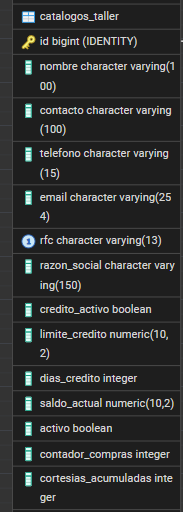
\includegraphics[width=0.5\linewidth]{imagenes/cstalogo talleres.png}
    \caption{Catalogo Talleres}
    \label{fig:tabla Talleres}
\end{figure}
Almacena la información detallada de los talleres externos vinculados al verificentro. Contiene datos de identificación legal, información de contacto y campos específicos para la gestión financiera, como límites de crédito, saldos actuales y el seguimiento de cortesías acumuladas por volumen de compra.

\subsection{Tabla Catálogos Técnico}
\begin{figure}[htbp]
    \centering
    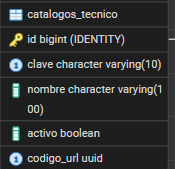
\includegraphics[width=0.5\linewidth]{imagenes/cstalogo tecnico.png}
    \caption{Catalogo Tecnicos}
    \label{fig:tabla Tecnicos}
\end{figure}
Entidad destinada al registro del personal técnico encargado de realizar las pruebas de verificación. Incluye una clave de identificación única por técnico y un campo \texttt{codigo\_url} de tipo UUID, utilizado para la generación de enlaces seguros o identificación digital dentro del sistema SIVEH.





\section{Tarjetas Kanban y Migraciones}
\label{anexo:kanban-migraciones}

\begin{center}
\begin{tabular}{|c|p{5.5cm}|l|}
\hline
\textbf{Tarjeta} & \textbf{Descripción} & \textbf{Estado Final} \\
\hline
K-01 & Schema inicial: subsistemas, usuarios, matrícula, evaluaciones, titulación & Desplegado \\
K-02 & Carga de catálogo de 7 subsistemas educativos & Desplegado \\
K-03 & Campos de auditoría en trabajos de carga & Desplegado \\
K-04 & Corrección de longitud en columna de estado & Desplegado \\
K-05 & Rol directivo y bitácora de auditoría & Desplegado \\
K-06 & Configuración de mapeo de columnas en Excel & Desplegado \\
K-07 & Renombrado y redefinición de roles del sistema & Desplegado \\
K-08 & Módulo de caracterización (discapacidad y etnia) & Desplegado \\
K-09 & Módulo de becas estudiantiles & Desplegado \\
K-10 & Catálogo de ciclos generacionales válidos & Desplegado \\
K-11 & Corrección semántica de campo docente & Desplegado \\
K-12 & Ajuste de campos nulos en titulación & Desplegado \\
K-13 & Desglose por sexo en becas y caracterización & Desplegado \\
\hline
\end{tabular}
\end{center}

\newpage
\nocite{*}
\printbibliography[heading=bibintoc, title={Referencias}]

\end{document}

